\documentclass[twocolumn]{aastex631}

% Packages you've added in
\usepackage{subcaption}
\usepackage{float} % Add the float package for additional float placement options
\usepackage{natbib} % Add the natbib package to handle undefined citations

\newcommand{\vdag}{(v)^\dagger}
\newcommand\aastex{AAS\TeX}
\newcommand\latex{La\TeX}
\newcommand{\code}[1]{\texttt{#1}}



\begin{document}

    \title{High Resolution Cross-Correlation Transmission Spectroscopy of KELT-20b}\footnote{Based on data acquired with the Potsdam Echelle Polarimetric and Spectroscopic Instrument (PEPSI) using the Large Binocular Telescope (LBT) in Arizona}

    \author[0009-0001-1459-3738]{Calder Lenhart}
    \affiliation{Department of Astronomy, The Ohio State University \\ 4055 McPherson Laboratory, 140 West 18th Avenue \\ Columbus, OH 43210}

    \author[0000-0002-5099-8185]{Marshall C. Johnson}
    \affiliation{Department of Astronomy, The Ohio State University \\ 4055 McPherson Laboratory, 140 West 18th Avenue \\ Columbus, OH 43210}

    \author{Ji Wang}
    \affiliation{Department of Astronomy, The Ohio State University \\ 4055 McPherson Laboratory, 140 West 18th Avenue \\ Columbus, OH 43210}

    \author[0000-0002-8823-8237]{Anusha Pai Asnodkar}
    \affiliation{Department of Astronomy, The Ohio State University \\ 4055 McPherson Laboratory, 140 West 18th Avenue \\ Columbus, OH 43210}

    \author{Sydney Petz}
    \affiliation{Department of Astronomy, The Ohio State University \\ 4055 McPherson Laboratory, 140 West 18th Avenue \\ Columbus, OH 43210}

    \author[0000-0002-6192-6494]{Klaus Stassmeier}
    \affiliation{Leibniz-Institut für Astrophysik Potsdam, An der Sternwarte 16 D-14482 Potsdam, Germany}

    \author[0000-0002-0551-046X]{Ilya Ilyin}
    \affiliation{Leibniz-Institut für Astrophysik Potsdam, An der Sternwarte 16 D-14482 Potsdam, Germany}


    %% Mark off the abstract in the ``abstract'' environment. 
    \begin{abstract}
        Ultra hot Jupiters (UHJs) are prime observational candidates owing to their proximity to their host stars. They have large radii with inflated envelopes, high temperatures, and short orbital periods --- allowing for frequent observations with strong signal clarity. Using the PEPSI high resolution spectrograph on the LBT, we present a complete inventory of detections, line velocities, and phase-resolved dynamics for atomic and molecular species in KELT-20b's atmosphere. We confirm previous detections of Fe I and Fe II, and Na I and report new tentative detections of Ni I, Ca I, Co I, and V I.
    \end{abstract}

    \keywords{}


    \section{Introduction}\label{sec:intro}

        High-resolution cross-correlation transmission spectroscopy (HRCCTS) of KELT-20b began in 2018 with detection of Na I and H$\alpha$\citep{CasasayasBarris2018}


    \section{Observations}\label{sec:Observations}
        We obtained our data with the Potsdam Echelle Polarimetric and Spectroscopic Instrument (PEPSI)\citep{Strassmeier2015} on the Large Binocular Telescope (LBT). We utilized the PEPSI CD III+V bandpass, with wavelength coverage of 4800--5441\AA\ and 6278--7419\AA\, henceforth referred to the blue arm and arm respectively, with resolution ${\mathcal{R} = 130000}$. We list the key observation parameters in deluxetable~\ref{tab:observation_details}.  %perhaps inlcude note about how many of the 23 spectra were in-transit vs out of transit
        We reduced this observation using the Spectroscopic Data Systems (SDS) Pipeline.

        \begin{deluxetable}{lc}
            \tablecaption{Observation details for 2019 May 4 transit.\label{tab:observation_details}}
            \tablehead{
                \colhead{\textbf{Parameter}} & \colhead{\textbf{Value}}
            }
            \startdata
            $N_{\text{spec}}$ & 23 \\
            Exp. Time (s) & 600 \\
            Airmass Range & 1.00--2.01 \\
            Phases Covered & $-0.023$--0.034 \\
            $S/N_{\text{blue}}$ & 288 \\
            $S/N_{\text{red}}$ & 308 \\
            \enddata
        \end{deluxetable}
        

        
    \section{Methodology}\label{sec:Methodology}

        \subsection{Model Spectra}\label{subsec:Model Spectra}
            We generate model transmission spectra, ranging from 3850--7500\AA\ with 0.01\AA\ spacing, with the \code{petitRADTRANS} package~\citep{petitRADTRANS}, as shown in Figure~\ref{fig:main-spectra}. These spectra encompass the PEPSI CD III+V bandpass. We assume stellar and planetary parameters from~\citet{Lund2017}, listed in Table~\ref{tab:parameters_summary}. We select a P-T profile given by Equation (29) of~\citet{Guillot2010} with best-fit parameters $\gamma = 30$ and $K_{IR} = 0.04$ as obtained in a grid search in~\citet{Johnson2023}. While these parameters were derived using emission spectra, transmission spectra are less sensitive to detailed vertical temperature structures~\citep{Kesseli2020}. Since our analysis concerns the atmosphere's kinematics as opposed to chemistry, we deem the same profile sufficient for this analysis. 
            We calculate volume mixing ratios (VMRs) for each species using the \code{PyFastChem} equilibrium chemistry model~\citep{Stock2018, Stock2022, Kitzmann2023}, assuming solar abundances~\citep{Asplund2021} and the aforementioned P-T profile. We assume that quenching, the mechanism by which atmospheric abundances diverge from those predicted by chemical equilibrium at a certain pressure, occurs at 1 bar. Thus, we approximate each species' VMR as equal to its maximum VMR at 1 bar, calculated by \code{PyFastChem}~\citep{Johnson2023,Petz2023}. Opacities were sourced from the~\code{petitRADTRANS} database, with missing entries supplemented from the DACE Opacity Database\footnote{\url{https://dace.unige.ch/opacityDatabase/}}, converted to \code{petitRADTRANS}-compatible format (P. Mollière, private communication).~\code{peitRADTRANS} sources its atomic opacities from the Kurucz line list, and we ensured the DACE opacities---Na I and Co I---came from the same line list.~\footnote{\url{http://kurucz.harvard.edu/}}
        
            \begin{deluxetable*}{l l c c}
                \tablecaption{This table summarizes the planetary and stellar parameters relevant to our analysis. Sources: 1:~\citet{Lund2017}; 2:~\citet{Johnson2023}.\label{tab:parameters_summary}}
                \tablehead{
                    \colhead{\textbf{Description}} & \colhead{\textbf{Parameter}} & \colhead{\textbf{Value}} & \colhead{\textbf{Source}}
                }
                \startdata
                \multicolumn{4}{c}{\textbf{Planetary Parameters}} \\
                \midrule
                Planet Radius & $R_P$ ($R_{\oplus}$) & 19.51 & 1 \\
                Planet Mass & $M_P$ ($M_{\oplus}$) & 1072 & 1 \\
                Equilibrium Temperature & $T_{\text{eq}}$ (K) & 2262 1 \\
                Orbital Period & $P$ (d) & 3.4741085 & 1 \\
                Epoch of Mid-Transit & $T_0$ (BJD\_TDB) & 2457485.74965 & 1 \\
                Planetary Radial Velocity Semi-amplitude & $K_p$ (km s$^{-1}$) & $169 \pm 6$ & 1 \\
                Systemic Velocity & $v_{\text{sys}}$ (km s$^{-1}$) & $-26.0$ & 2 \\
                Projected Equatorial Rotational Velocity & $v \sin i_P$ (km s$^{-1}$) & 2.5 & 1 \\
                Infrared Opacity & $\kappa_{\text{IR}}$ & 0.04 & 2 \\
                Ratio of Optical to Infrared Opacities & $\gamma$ & 30 & 2 \\
                Reference Pressure & $P_0$ (bar) & 1 & 2 \\
                Atmospheric Abundance of H & $X_{\text{H}_2}$ & 0.7496 & 2 \\
                Atmospheric Abundance of He & $X_{\text{He}}$ & 0.2504 & 2 \\
                Volume Mixing Ratio of H$^-$ & VMR (H$^-$) & $1 \times 10^{-9}$ & 2 \\
                \midrule
                \multicolumn{4}{c}{\textbf{Stellar Parameters}} \\
                \midrule
                Stellar Radius & $R_{\ast}$ (Re) & 1.565 & 1 \\
                Stellar Mass & $M_{\ast}$ (Me) & 1.76 & 1 \\
                Stellar Effective Temperature & $T_{\text{eff}}$ (K) & 8720 & 1 \\
                Metallicity & $[$Fe/H$]$ & $-0.29$ & 1 \\
                \enddata
            \end{deluxetable*}
            
            We analyzed species presented in three previous spectral surveys of UHJs, ESPRESSO observations of WASP-76b in~\citet{Kesseli2022}, HARPS-N observations of KELT-9b in~\citet{Hoeijmakers2019}, and PEPSI observations of this planet in~\citet{Petz2023}. Considering HARPS-N's bandpass is 3830--6900\AA\~\citep{Cosentino2012} and ESPRESSO's is 3782--7887\AA\~\citep{Pepe2021}, we concluded that these studies provide a comprehensive overview of potential atmospheric constituents for KELT-20b. Consequently, we focused our search on the species identified as observable in these analyses.
            
        \subsection{Data Preparation}\label{subsec:Data Preparation}
            The following procedure is nearly identical to that of~\citep{Johnson2023} and~\citep{Petz2023}. First, we import the flux values for each spectrum recorded, then regrid the fluxes to common wavelength values for each spectrum. Next, we flatten both arms of the time-series spectra by subtracting off the median flux from each, yielding residual spectra with stellar lines and time-invariant telluric lines removed. Next, we remove systematics from the spectra. Our systematics correction method is unique in that it employs both the~\code{molecfit} package~\citep{Smette2015, Kausch2015} and a modified version of the \code{PySysRem}~\footnote{https://github.com/stephtdouglas/PySysRem} package that accepts PEPSI data.~\code{molecfit} corrects for tellurics by generating synthetic absorption lines specific to time and location of observation and removing them from obtained spectra. The SYSREM detrending algorithm~\citep{Tamuz2005} fits and removes systematic effects, with the number of systematics to correct for ($N_{\mathrm{Sys}}$) and the number of SYSREM iterations ($N_{\mathrm{Iter}}$) being the relevant input parameters. As determined in~\citet{Johnson2023}, applying both methods yields increased significance of retrieved signals than either alone. We first use~\code{molecfit} to fit and remove telluric lines in the red arm spectra only, as the blue arm is absent of significant tellurics~\citep{Smette2015}. Next, we apply SYSREM to the residual spectra, empirically determining the number of iterations to apply to the spectra, the amount which yields the greatest recovered SNR in each species, as shown in Table~\ref{tab:sysrem_and_vmr}.

        \begin{table*}[ht]\label{tab:sysrem_and_vmr}
            \centering
            \begin{tabular}{lcccc}
                \textbf{Species} & $\textbf{N}_{\mathrm{Sys},\text{Red}}$ (Non-telluric) & $\textbf{N}_{\mathrm{Sys},\text{Red}}$ (Telluric) & $\textbf{N}_{\mathrm{Sys},\text{Blue}}$ & VMR \\
                \hline
                Fe I & 5 & 5 & 6 & $5.39 \times 10^{-5}$ \\        
                Fe II & 5 & 5 & 5 & $5.39 \times 10^{-5}$ \\
                Na I & 0 & 10 & 2 & $2.94 \times 10^{-6}$ \\
                Co I & 0 & 10 & 5 & $1.67 \times 10^{-7}$ \\
                V I & 2 & 5 & 8 & $5.62 \times 10^{-9}$ \\
                Ca I & 0 & 10 & 5 & $2.10 \times 10^{-8}$ \\
            \end{tabular}
            
            \caption{Shows the optimal SYSREM iterations, $N_{\mathrm{Sys}}$, for systematics reduction for each species meeting the tentative detection threshold. We bin the telluric and non-telluric contaminated wavelength regions, finding the best $N_{\mathrm{Sys}}$ for each. Note that the blue arm does not contain any tellurics, so it only contains one $N_{\mathrm{Sys}}$ parameter, for non-telluric regions.}
            

        \end{table*}

        \subsection{Cross-correlation}
            With data preparation complete, we cross-correlate model and observed spectra in the stellar rest frame, with the same procedure as described in~\citet{Johnson2023}. To find the peak SNR of each spectrum in our dataset, we divided the flux values by their corresponding error values, then selected the 90th percentile value. We compute per-spectrum CCF weights by regridding the Doppler shift-corrected spectra wavelengths to the template wave wavelengths, then multiplying the per-spectrum SNR with the difference between the maximum flux value of the regridded template spectrum and the flux values of the regridded template itself. The cross-correlation procedure is adapted from the BANZAI-NRES package~\citep{McCully2022}. With each spectrum cross-correlated, we then interpolate the cross-correlation function and its uncertainty for the given radial velocity shift corresponding to $K_p$. We sum over all spectra, multiplying each by its corresponding CCF weight, then median subtract. Finally, we standardized the now-combined CCF amplitude with the metric of the detection strength being the standard deviation of the CCF at $|v_{sys}| > 100 km/s$.
            
            Next, we shift the CCFs into the planetary rest frame and stack the red and blue arm CCFs separately. With a ${K_p-v_{sys}}$ map generated, we search for a CCF peak over a grid of $K_p$ values ranging from $50-350$ kms$^{-1}$ in steps of $1.0$ kms$^{-1}$. These maps are shown for each species within and exceeding the ${3\sigma}-{5\sigma}$ tentative detection window in Figure~\ref{fig:main-CCFs}. The VMRs for species meeting or exceeding the tentative detection window are shown in Table 1, as computed with the methodology described in Section~\ref{subsec:Model Spectra}.

        \subsection{Doppler Shadow Removal}
            As the planet crosses the stellar disk, the disk-integrated rotationally-broadened stellar absorption lines are deformed, a phenomenon known as the Rossiter-McLaughlin (RM) effect. When dividing each in-transit spectra by the out-of-transit spectra to isolate the atmospheric signal, the deformed lines cause an artifact on the CCF at the radial velocity corresponding to to the stellar disk being blocked by the transiting planet at the time of exposure, referred to as the Doppler shadow. We must correct for this obfuscation of the planetary signal in the CCF, as it decreases the recovered SNR and can alter the calculated radial velocity of each detection. KELT-20b's orbit is well-aligned ($\lambda = 3.4 \pm 2.1 ^{\circ}$) with its fast-rotating host star's projected-spin axis~\citep{Lund2017}, causing a strong RM effect. We correct for the RM effect using a Doppler shadow model, described in detail in~\citep{Johnson2016} and further discussed in~\citep{Johnson2014, Johnson2017}. In brief, we begin by dividing the stellar disk into a surface elements defined by $n \times n$ Cartesian grid, finding the fraction of each exposure time that grid spaces are obscured or partially obscured. We assume solid body rotation and a Gaussian profile in each surface element, scaled by a quadratic limb darkening coefficient. We also neglect the broadening effects of macroturbulence and gravity darkening~\citet{Johnson2016}. We scale the line profile contribution by each obscured surface element by this fraction, then convolve the line profiles with the instrumental line profile, a Gaussian. Finally, we subtract the line profile by the out-of-transit line profile, yielding the time-series CCF contribution from only the transiting planet, the Doppler Shadow. Our model outputs a normalized line profile, so we must rescale the model to match the CCF amplitudes. We run a grid search with the the Doppler shadow model scaling as the free parameter, with root-mean-square error as the goodness-of-fit metric. We select the best fit scaled Doppler shadow model, then subtract it from the CCFs. Finally, we again mean subtract and normalize each CCF, then combine arms into a single set of CCFs.
            
            \begin{figure*}[ht!]\label{fig:raw-CCFs}
            % Row 1
                \begin{subfigure}[b]{0.333\textwidth}\label{fig:raw-ccf-before-Fe-blue}
                    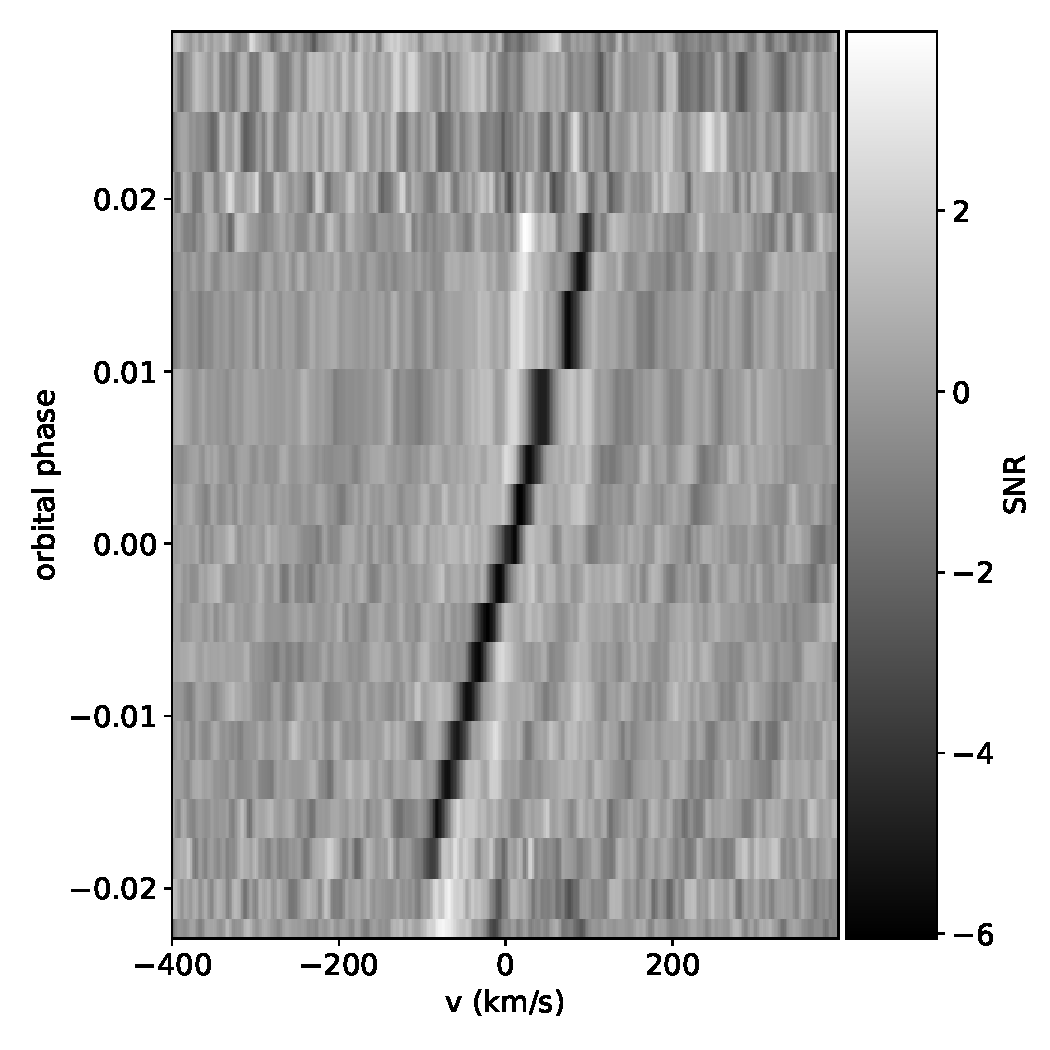
\includegraphics[width=\textwidth]{plots/raw-ccf-before/KELT-20b.20190504.Fe.blue.CCFs-raw.pdf}
                \end{subfigure}

                \begin{subfigure}[b]{0.333\textwidth}\label{fig:raw-ccf-after-Fe-blue}
                    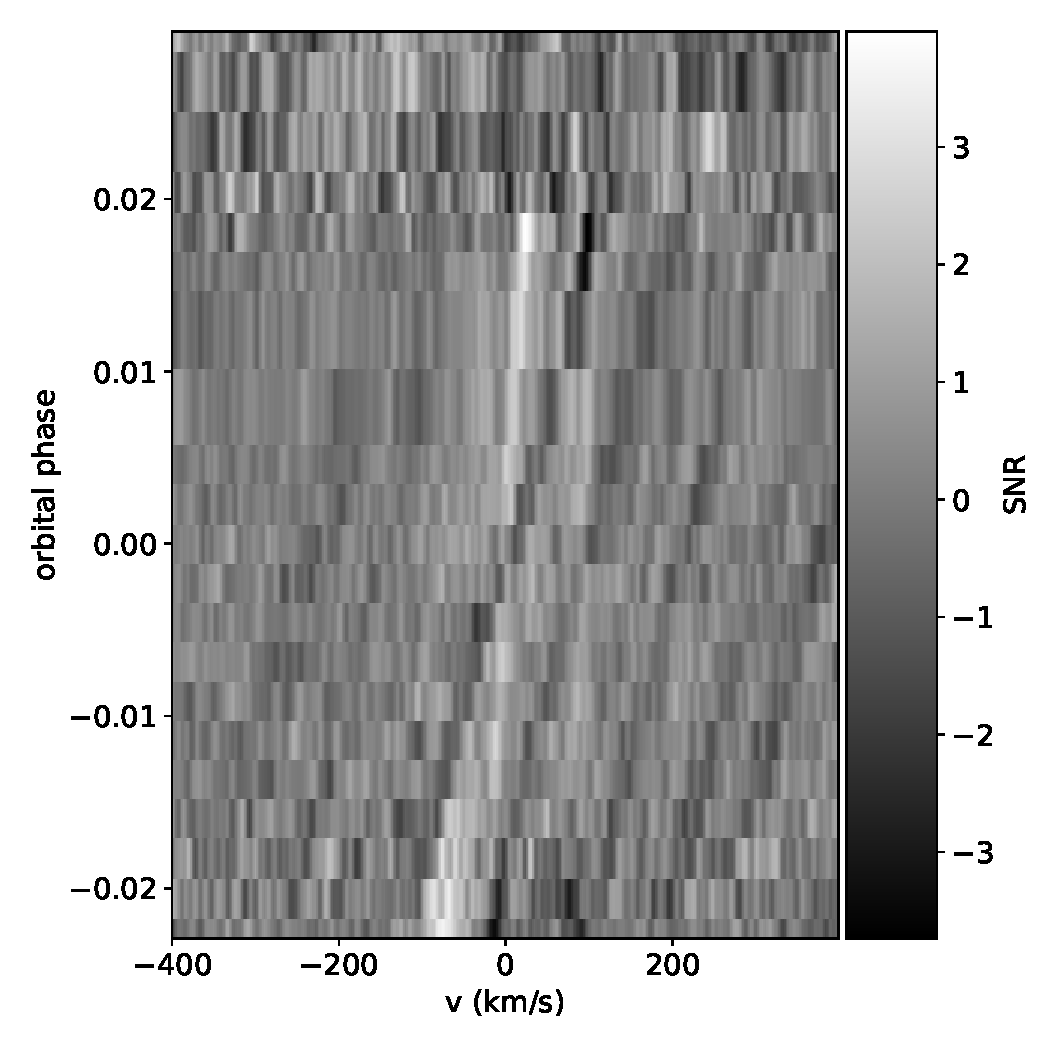
\includegraphics[width=\textwidth]{plots/raw-ccf-after/KELT-20b.20190504.Fe.blue.CCFs-raw.pdf}
                \end{subfigure}
            
            \caption{Removal of the Doppler shadow in the blue arm CCF of Fe I. \textit{Left panel}: CCF of in-transit exposures showing Doppler Shadow (dark streak) intersecting with the radial velocity signal (bright streak).~\textit{Right panel}: Residual CCF after the subtracting off the Doppler shadow.}

            \end{figure*}
                
        \subsection{Line Velocities}\label{subsec:Line Velocities}
            We select the point of maximum SNR on the ${K_p-v_{sys}}$ map, both for the individual arms and the combined arms, effectively isolating the 1D CCF absorption lines with a constant ${K_p}$ corresponding to maximum SNR.

            The fitting procedure is as follows: Working in the ${K_p-RV}$ space of a single time-series CCF, we loop over a range of possible $K_p$ values: $50$-$350$. For each $K_p$ slice, we search through the peaks along the one-dimensional $RV$ array in descending order, selecting the greatest peak with an $|RV| \leq 15$ kms$^{-1}$. We then fit the Gaussian curve, our initial guess for its center $\mu = RV$. This procedure automatically filters out peaks at nonphysical velocities that may arise due to aliasing.
            We select the fit parameters corresponding to the $K_p$ slice hosting the peak CCF amplitude across the entire $K_p-v_{sys}$ map, reporting the species velocity $v_{sys} = \mu$ and its detection significance $SNR$ equal to the amplitude of the Gaussian in Table~\ref{tab:results-summary}.
            
            We repeat this fitting procedure for each in-transit time-series CCF, but instead selecting the fit parameters that correspond to the $K_p$ slice equal to the expected $K_p$ of KELT-20b per the ephemeris in Table~\ref{tab:parameters_summary}. We then plot the species' $v_{sys}$ as a function of orbital phase, effectively observing its line velocity change over the course of each in-transit exposure. The described plots for each species are in Figure~\ref{fig:main-CCFs}. 

        \subsection{Assessing Detection Validity}\label{subsec:Assessing Detection Results}
            With a ${K_p-v_{sys}}$ map 2D CCF, 1D CCF with Gaussian fit at peak SNR $K_p$ slice, and a phase-resolved line profile center during transit, we have a comprehensive profile of each atomic species detected in KELT-20b's atmosphere. We heuristically assess the detection validity by noting the location and magnitude of the peak signal on the ${K_p-v_{sys}}$ map, and checking three criteria in order: A ${3\sigma}$ SNR peak, a standard shape within ${K_p-v_{sys}}$ space, and a $v_{sys}$ within a physical range of line velocities. Aside from this procedure, we must also consider aliasing between the search species and strong lines corresponding to other species in the spectrum, as described in~\citet{Borsato2023}. In the 1D CCFs, these artifacts manifest as peaks at both visually detectable nonphysical $v_{sys}$ values, and peaks that overlap with the true absorption signal.
            % plot of example telluric corrections by molecfit
            
            % plots showing petitRADTRANS-generated model spectra for each species meeting tentative detection threshold
            
    \section{Results}\label{sec:Results}
            
        \begin{table*}\label{tab:results-summary}
            \centering
            \caption{Comparative analysis of detected and tentatively detected species across different studies, including new findings.}
            
            {\footnotesize % Slightly reduce the font size
            \setlength\tabcolsep{4pt} % Adjust the spacing between columns to be tighter
            \begin{tabular}{lcccc}
                \hline
                & Species & SNR & $V_{sys}$ & $(K_p)$ \\
                \hline
                \textbf{This Work} & Fe I & 10.16 & -0.81 & 188 \\
                & Fe II & 18.73 & 0.72 & 163 \\
                & Na I & 3.00 & 3.75 & 211 \\
                & Co I & 2.94 & -1.99 & 110 \\
                & V I & 3.13 & -3.79 & 220 \\
                \citep{CasasayasBarris2020} & Fe II & --- & -2.8 $\pm$ 0.8 & --- \\
                & Na I & --- & -3.1 $\pm$ 0.9 & --- \\
                & $H_{\alpha}$ & --- & -3.0 $\pm$ 1.2 & --- \\
                \citep{Hoeijmakers2020} & Na I & --- & -3.2 $\pm$ 0.7 & --- \\
                & $H_{\alpha}$ & --- & -4.5 $\pm$ 0.5 & --- \\
                \citep{Nugroho2020} & Fe I (3000K) & 14.30 & -3.6  $\pm$ 0.3 & 200.1 $\pm$ 5.2 \\
                & Fe II (3000K) & 14.61 & -1.4 $\pm$ 0.2 & 165.0 $\pm$ 3.5 \\
                & Na I D (3000K) & 7.72 & -1.4 $\pm$ 0.7 & 180.0 $\pm$ 11.8 \\
                \citep{Kasper2022} & --- & 5.4 & $2.0^{+2.0}_{-2.0}$ & $173.0^{+6.5}_{-5.0}$ \\
                \citep{Sicilia2022} & $H_{\alpha}$ & --- & $-5.2^{+1.8}_{-1.7}$ & $156.3^{+28.5}_{-27.0}$ \\
                & Na I D_1 & --- & $-3.8^{+0.7}_{-0.7}$ & $192.5^{+12.4}_{-13.5}$ \\
                & Na I D_2 & --- & $-3.7^{+0.9}_{-0.9}$ & $170.0^{+14.9}_{-13.5}$ \\
                \citep{BelloArufe2022} & Fe II & 5.3 & -20$^{+2}_{-6}$ & 120$^{+78}_{-46}$ \\
                
                \hline

            \end{tabular}}
            
        \end{table*}

        \begin{figure*}[ht!]
            % Row 1
            \begin{subfigure}[b]{0.333\textwidth}\label{fig:2d-ccf-Fe-combined}
                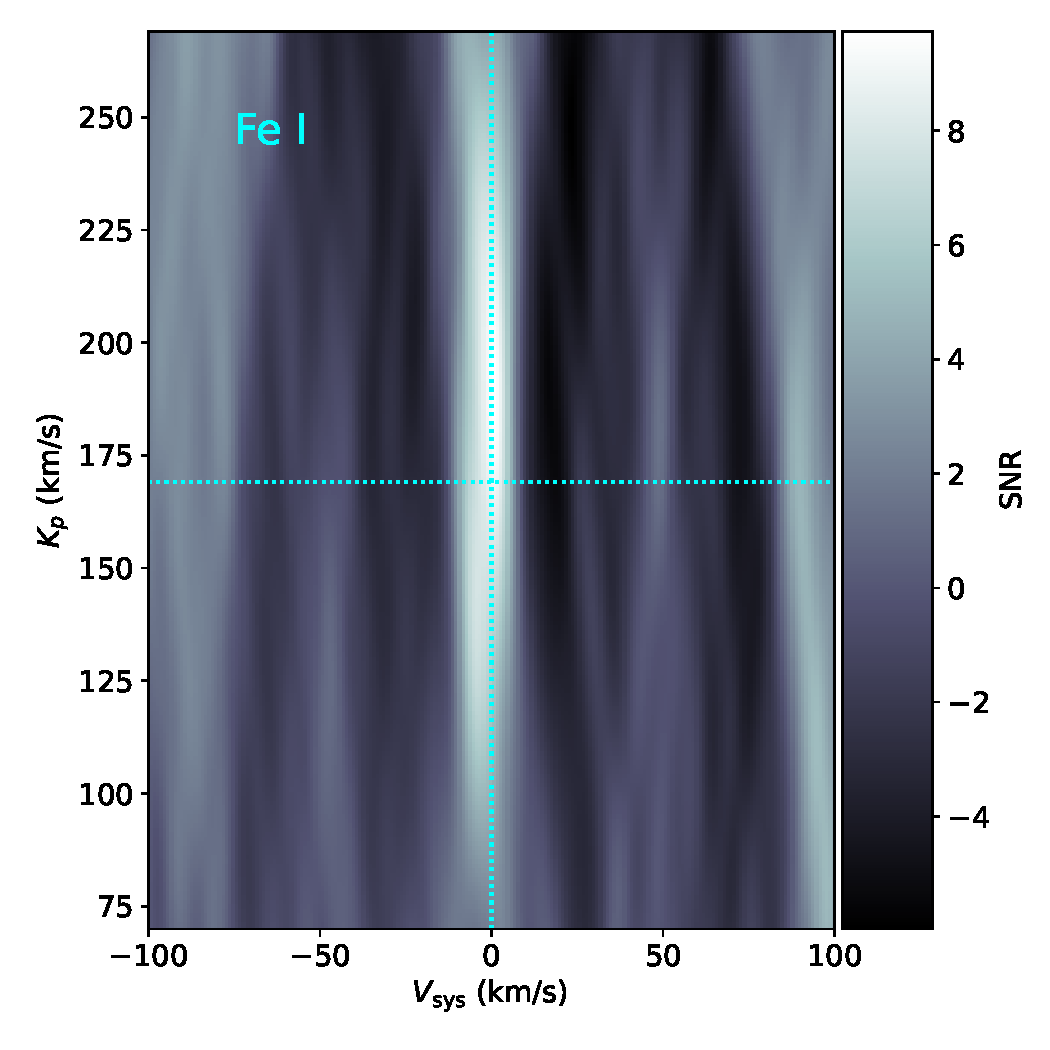
\includegraphics[width=\textwidth]{plots-updated/kp-vsys-map/combined/KELT-20b.20190504.combined.Fe.CCFs-shifted.pdf}
                
            \end{subfigure}
            \begin{subfigure}[b]{0.333\textwidth}\label{fig:1d-ccf-Fe-combined}
                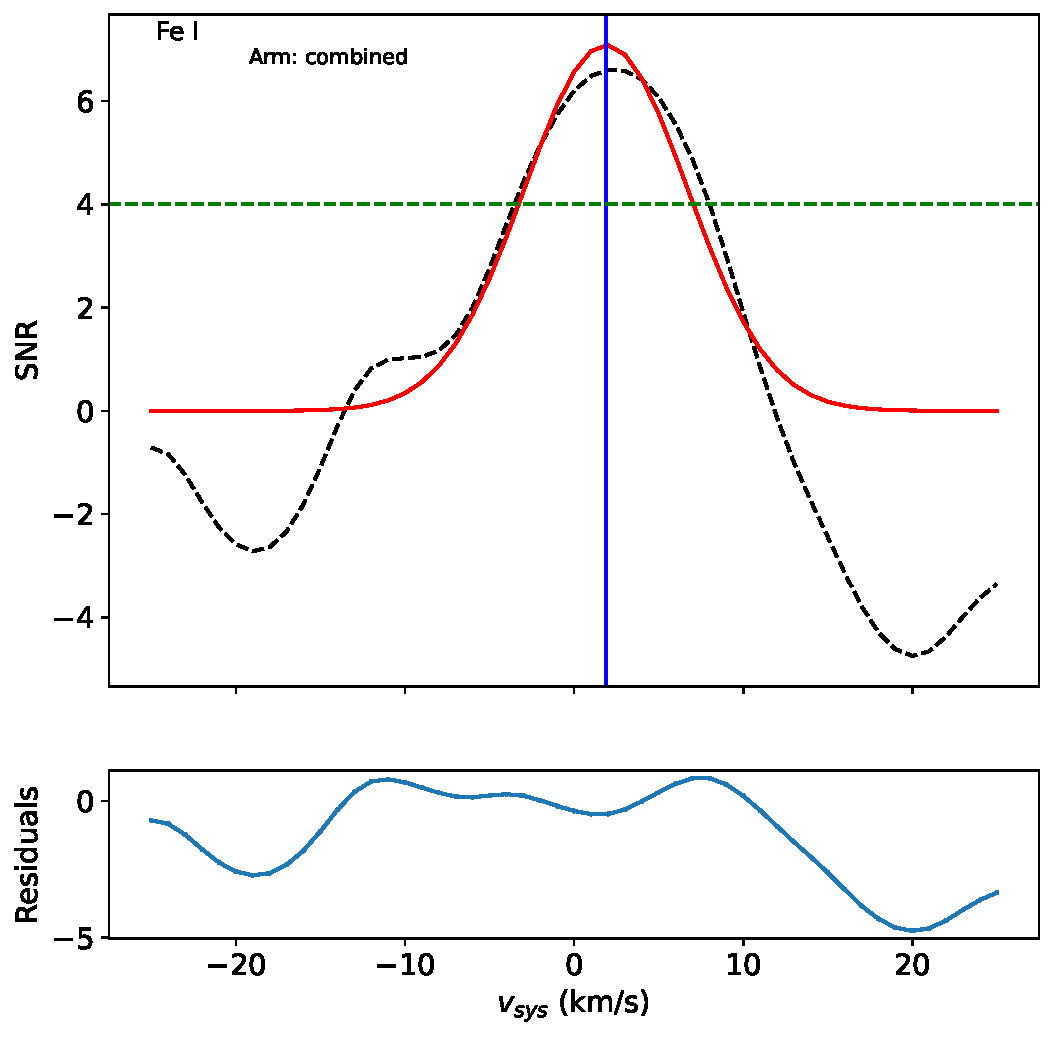
\includegraphics[width=\textwidth]{plots-updated/line-profile/combined/KELT-20b.20190504.combined.Fe.SNR-Gaussian.pdf}
                
            \end{subfigure}
            \begin{subfigure}[b]{0.333\textwidth}\label{fig:wind-chars-Fe-combined}
                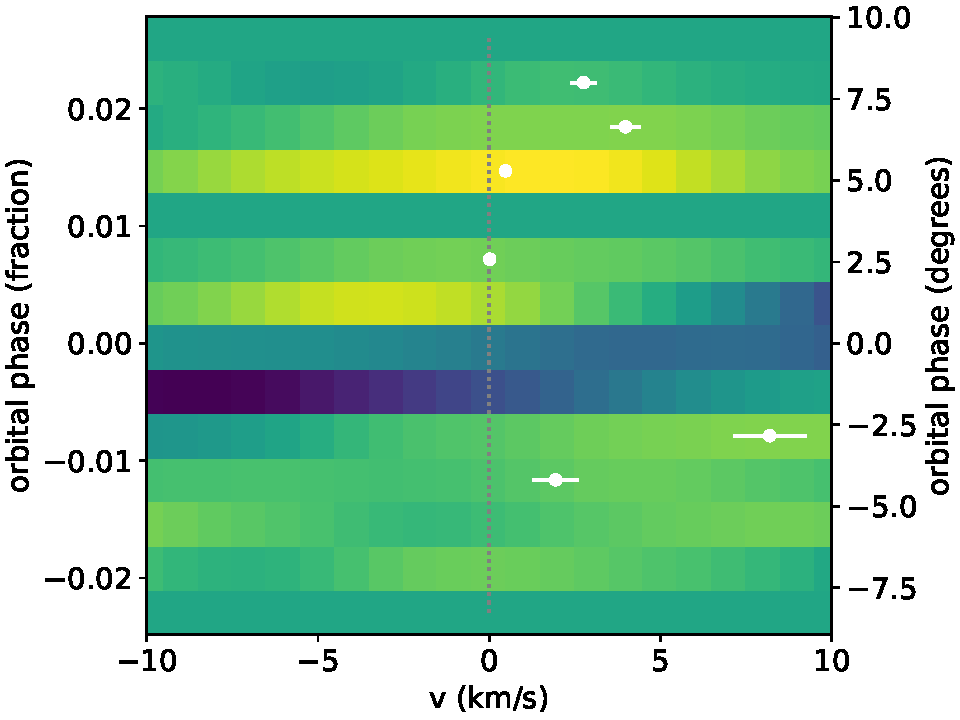
\includegraphics[width=\textwidth]{plots-updated/line-velocity/binned/pcolor/points/KELT-20b.Fe.phase-binned+RVs.pdf}
                
            \end{subfigure}

            \begin{subfigure}[b]{0.333\textwidth}\label{fig:2d-ccf-Fe+-combined}
                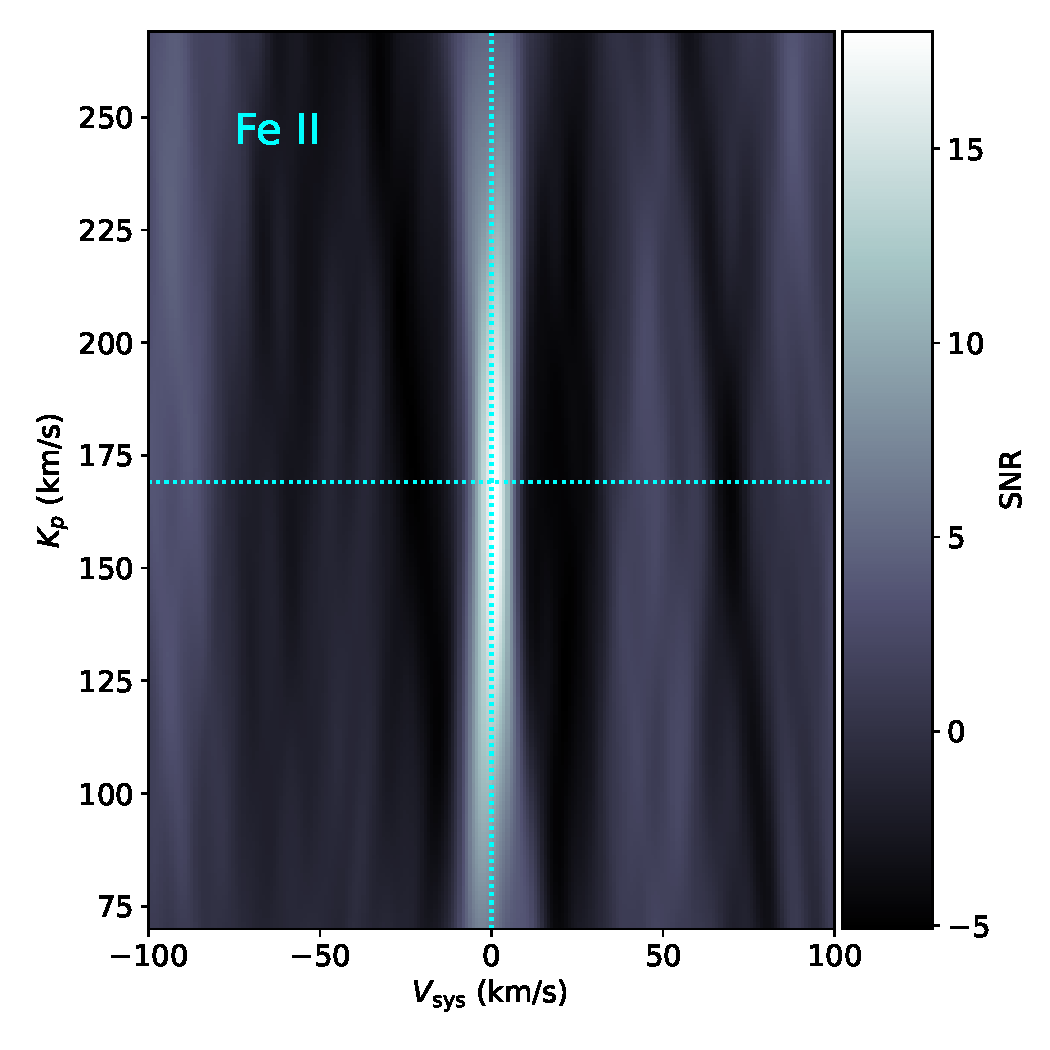
\includegraphics[width=\textwidth]{plots-updated/kp-vsys-map/combined/KELT-20b.20190504.combined.Fe+.CCFs-shifted.pdf}
                
            \end{subfigure}
            \begin{subfigure}[b]{0.333\textwidth}\label{fig:1d-ccf-Fe+-combined}
                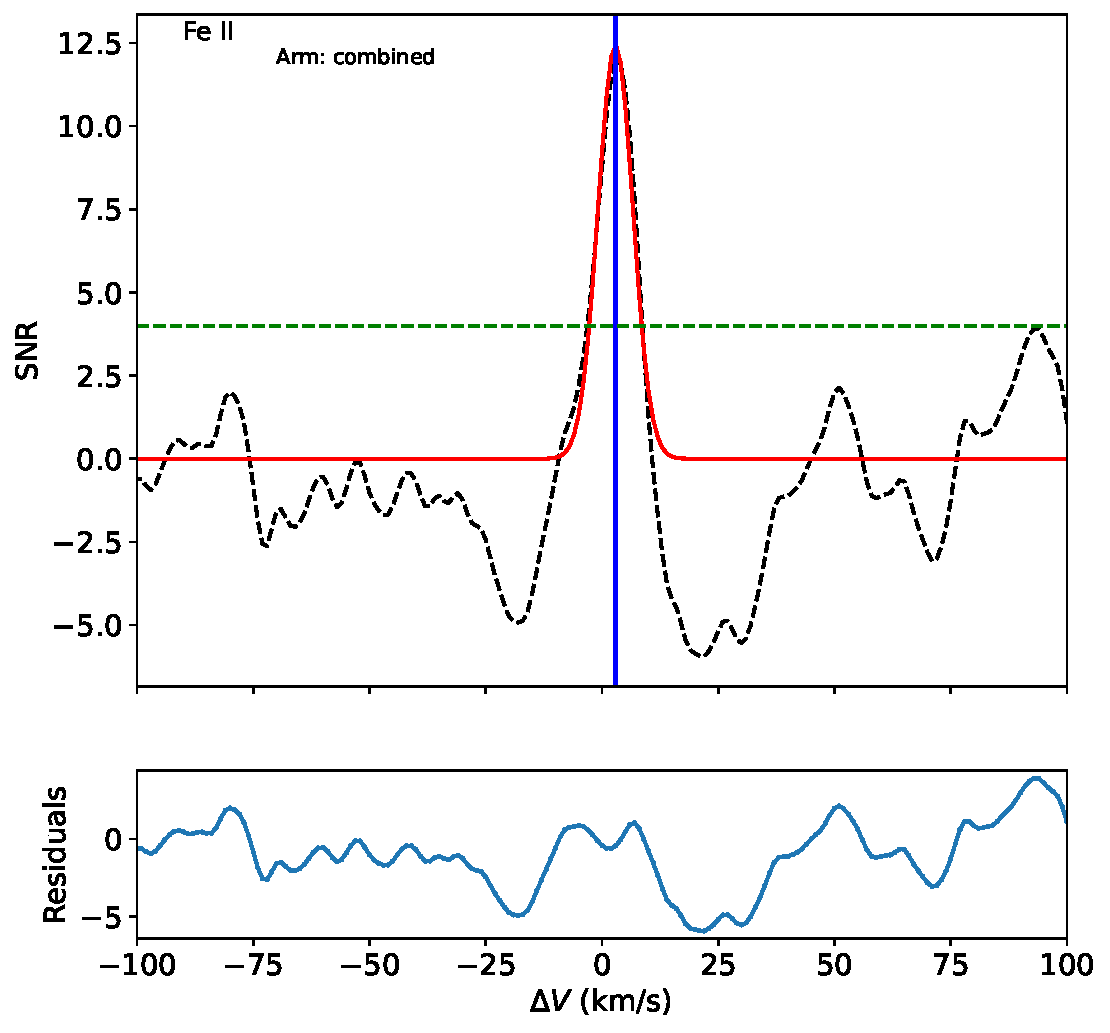
\includegraphics[width=\textwidth]{plots-updated/line-profile/combined/KELT-20b.20190504.combined.Fe+.SNR-Gaussian.pdf}
                
            \end{subfigure}
            \begin{subfigure}[b]{0.333\textwidth}\label{fig:wind-chars-Fe+-combined}
                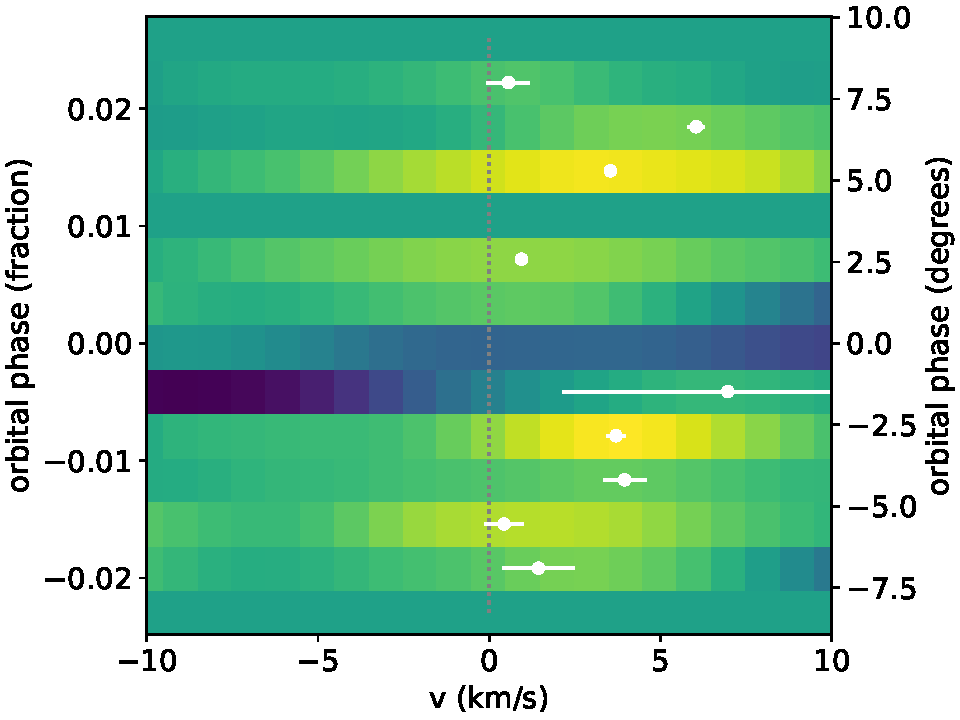
\includegraphics[width=\textwidth]{plots-updated/line-velocity/binned/pcolor/points/KELT-20b.Fe+.phase-binned+RVs.pdf}
                
            \end{subfigure}

            \begin{subfigure}[b]{0.333\textwidth}\label{fig:2d-ccf-Na-combined}
                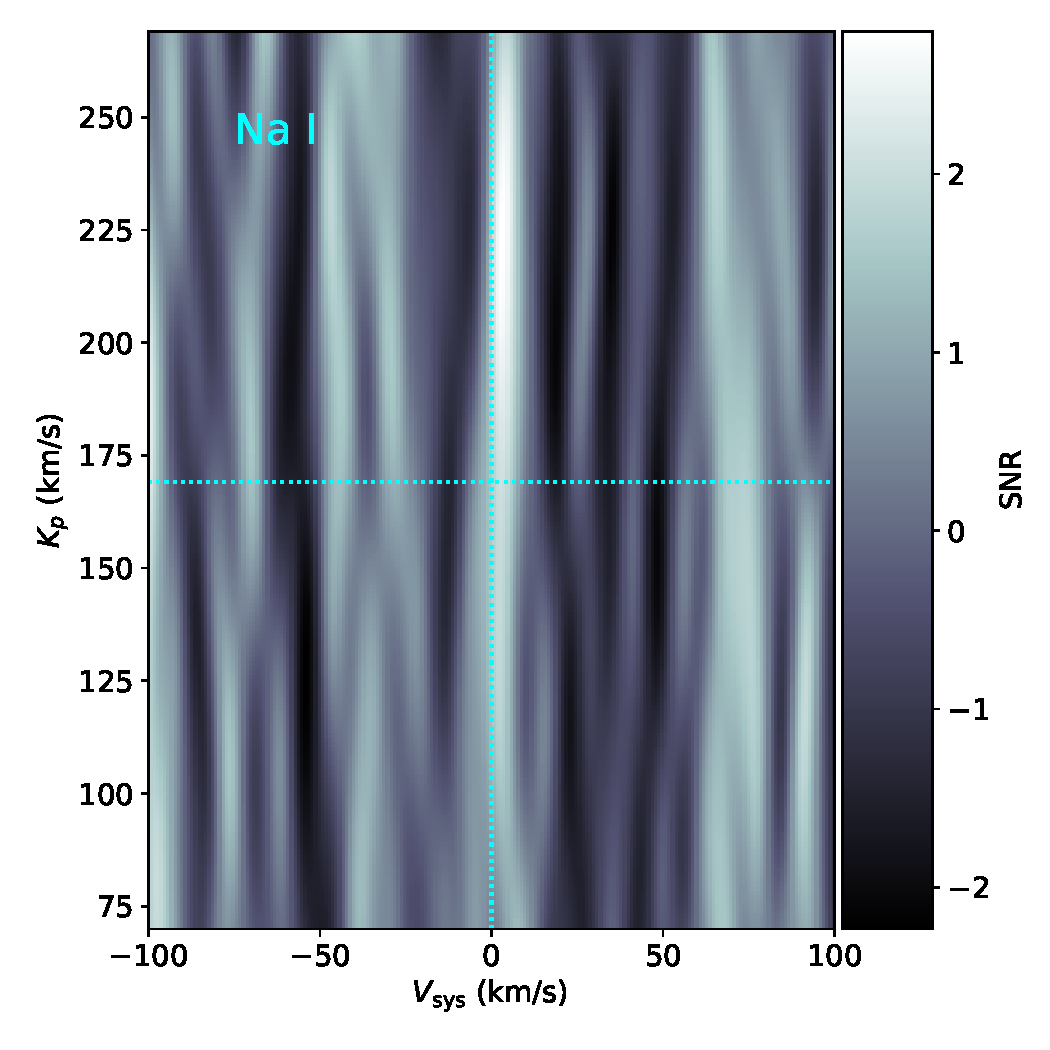
\includegraphics[width=\textwidth]{plots-updated/kp-vsys-map/combined/KELT-20b.20190504.combined.Na.CCFs-shifted.pdf}
                
            \end{subfigure}
            \begin{subfigure}[b]{0.333\textwidth}\label{fig:1d-ccf-Na-combined}
                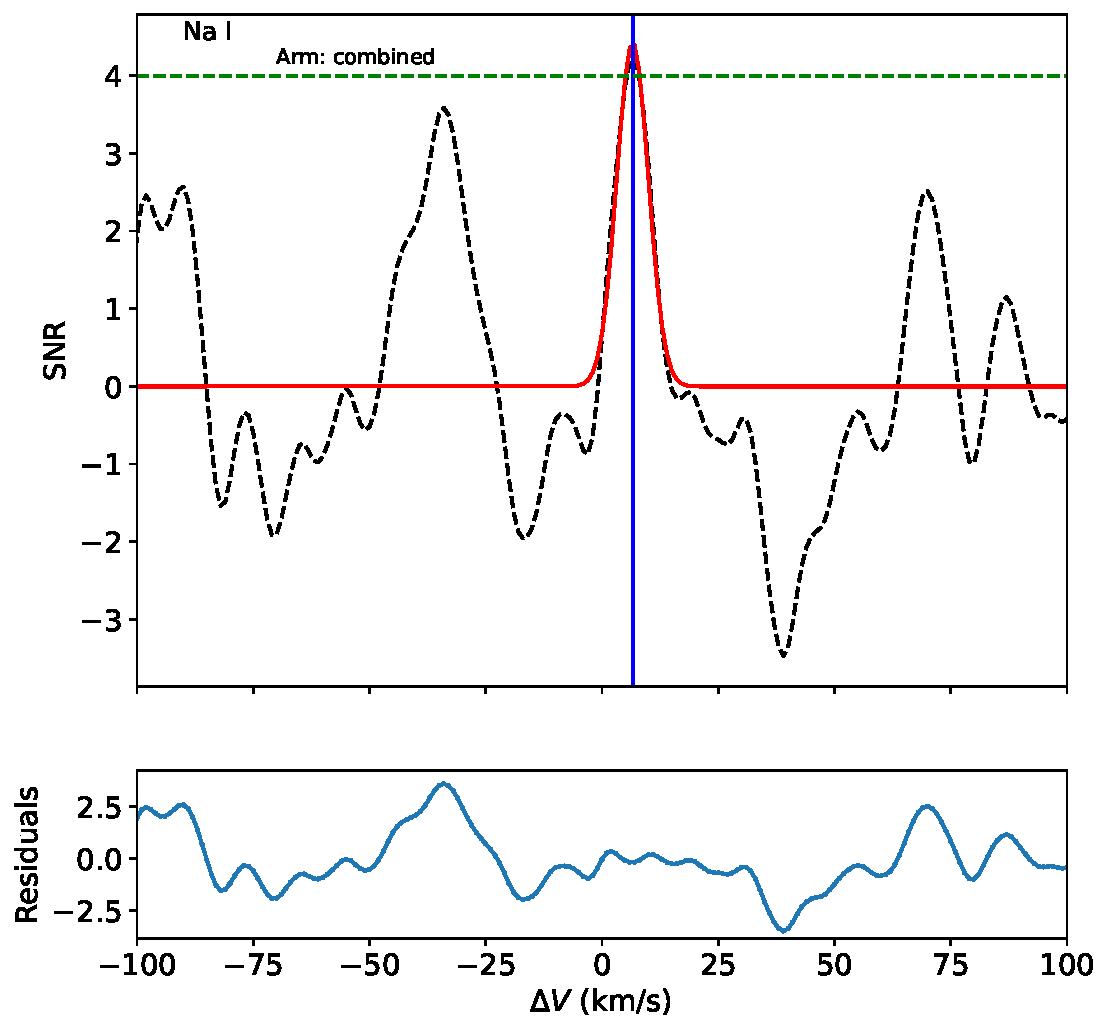
\includegraphics[width=\textwidth]{plots-updated/line-profile/combined/KELT-20b.20190504.combined.Na.SNR-Gaussian.pdf}
                
            \end{subfigure}
            \begin{subfigure}[b]{0.333\textwidth}\label{fig:wind-chars-Na-combined}
                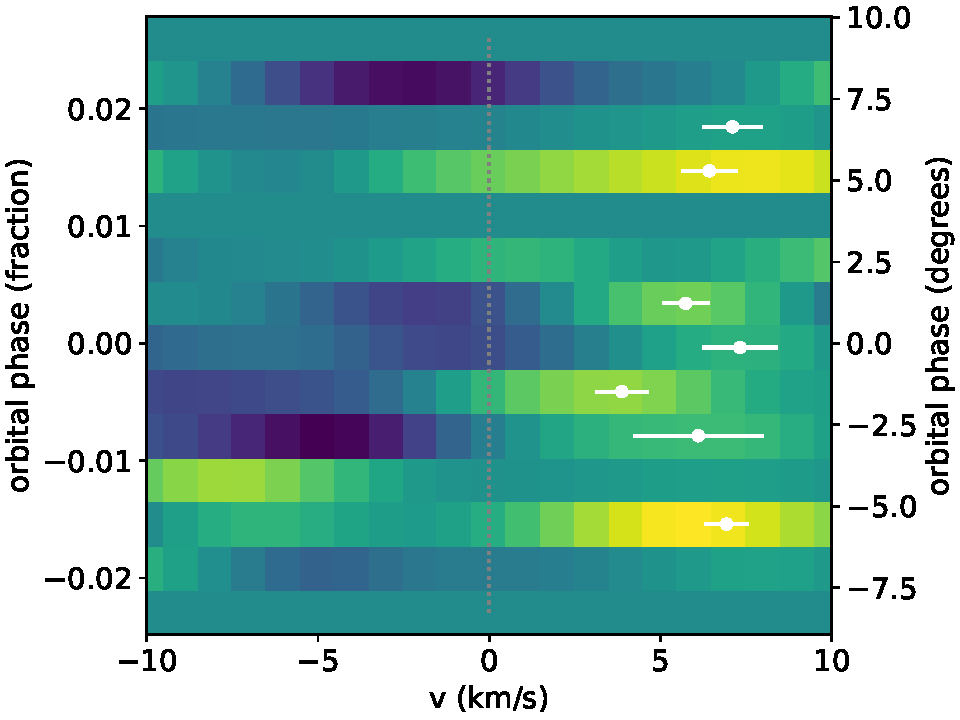
\includegraphics[width=\textwidth]{plots-updated/line-velocity/binned/pcolor/points/KELT-20b.Na.phase-binned+RVs.pdf}
                
            \end{subfigure}

        \end{figure*}
        
        \begin{figure*}[ht!]\label{fig:main-CCFs}
            \ContinuedFloat%

            \begin{subfigure}[b]{0.333\textwidth}\label{fig:2d-ccf-Co-combined}
                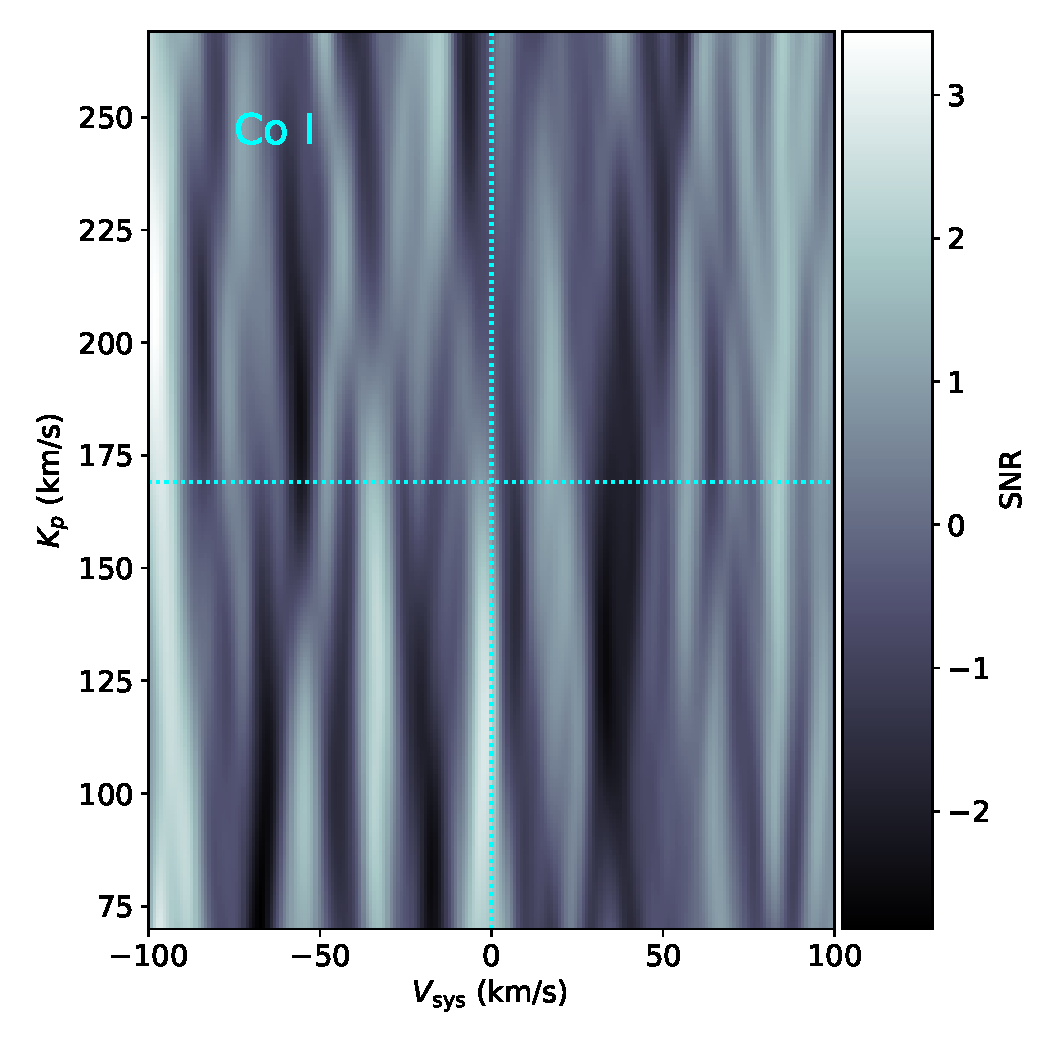
\includegraphics[width=\textwidth]{plots-updated/kp-vsys-map/combined/KELT-20b.20190504.combined.Co.CCFs-shifted.pdf}
                
            \end{subfigure}
            \begin{subfigure}[b]{0.333\textwidth}\label{fig:1d-ccf-Co-combined}
                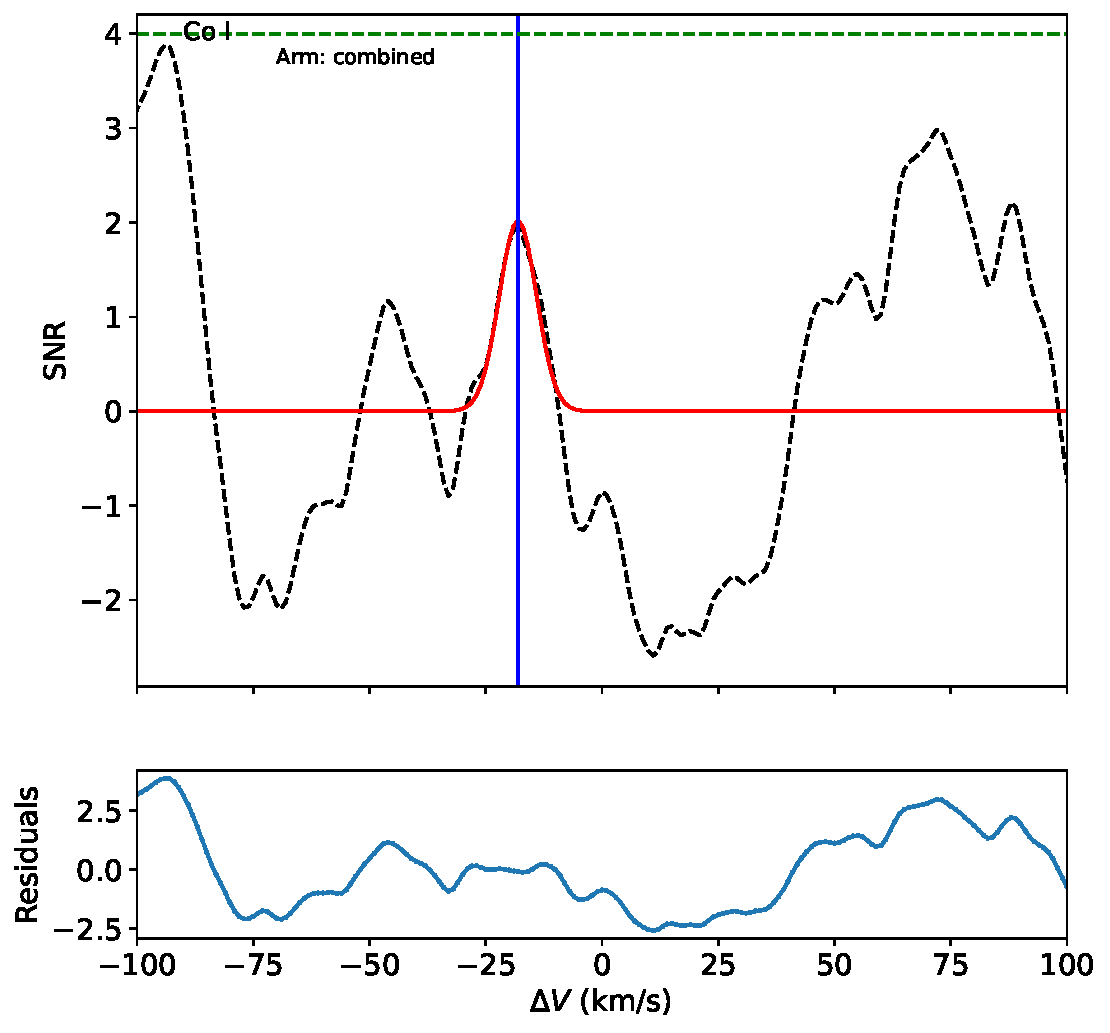
\includegraphics[width=\textwidth]{plots-updated/line-profile/combined/KELT-20b.20190504.combined.Co.SNR-Gaussian.pdf}
                
            \end{subfigure}
            \begin{subfigure}[b]{0.333\textwidth}\label{fig:wind-chars-Co-combined}
                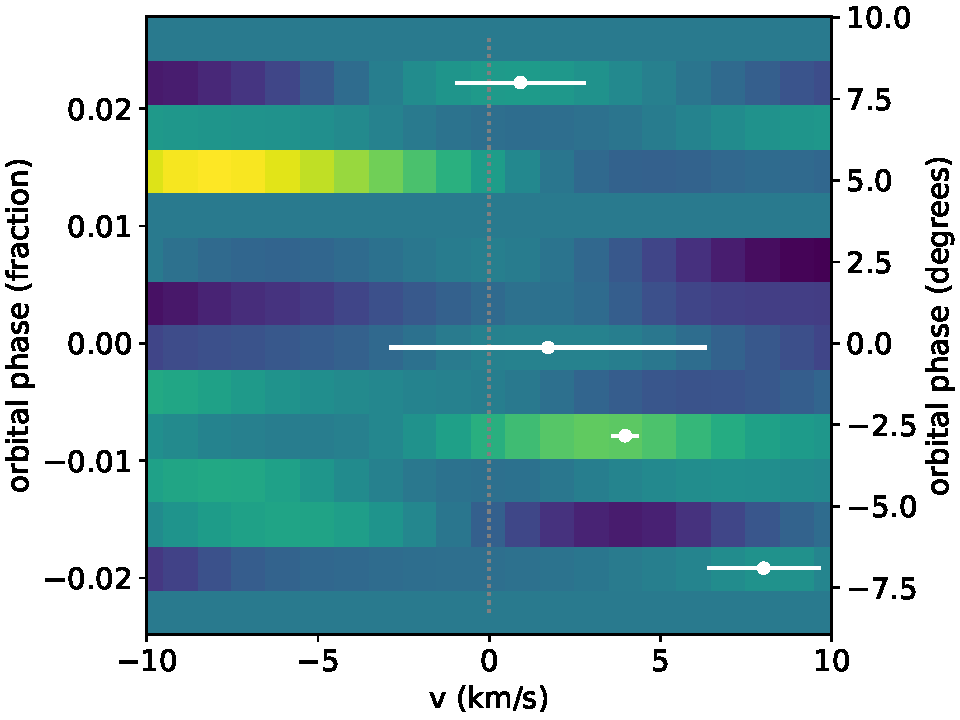
\includegraphics[width=\textwidth]{plots-updated/line-velocity/binned/pcolor/points/KELT-20b.Co.phase-binned+RVs.pdf}
                
            \end{subfigure}

            \begin{subfigure}[b]{0.333\textwidth}\label{fig:2d-ccf-V-combined}
                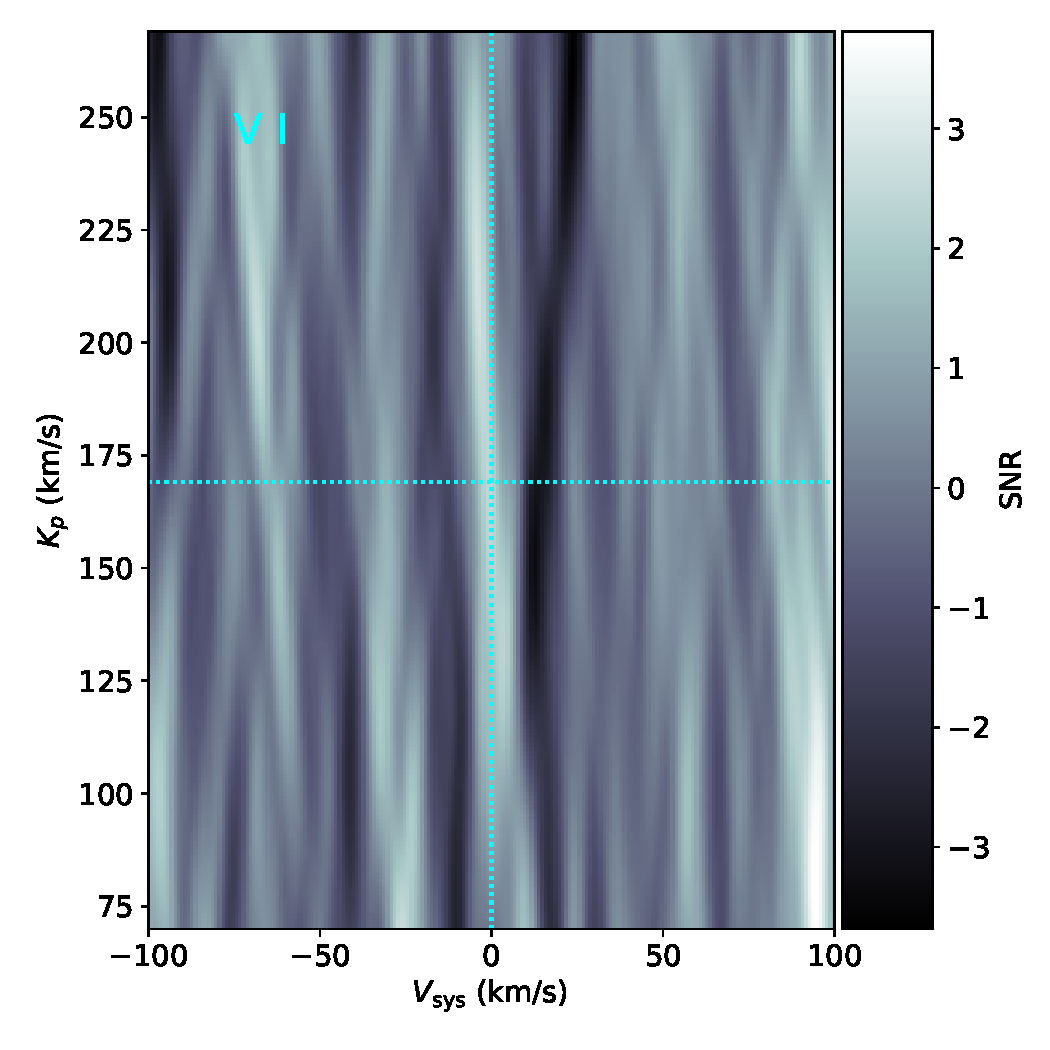
\includegraphics[width=\textwidth]{plots-updated/kp-vsys-map/blue/KELT-20b.20190504.blue.V.CCFs-shifted.pdf}
                
            \end{subfigure}
            \begin{subfigure}[b]{0.333\textwidth}\label{fig:1d-ccf-V-combined}
                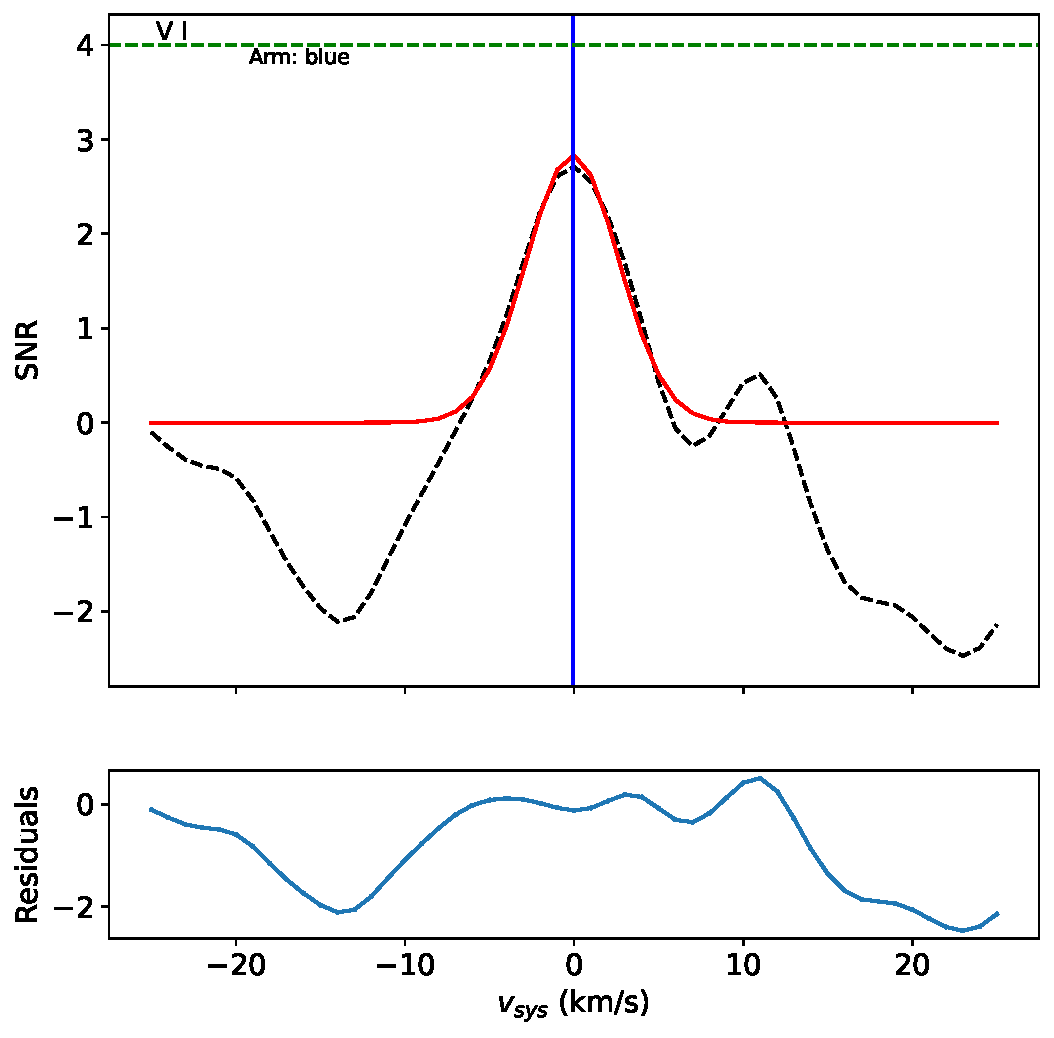
\includegraphics[width=\textwidth]{plots-updated/line-profile/blue/KELT-20b.20190504.blue.V.SNR-Gaussian.pdf}
                
            \end{subfigure}
    
            \begin{subfigure}[b]{0.333\textwidth}\label{fig:2d-ccf-Ca-combined}
                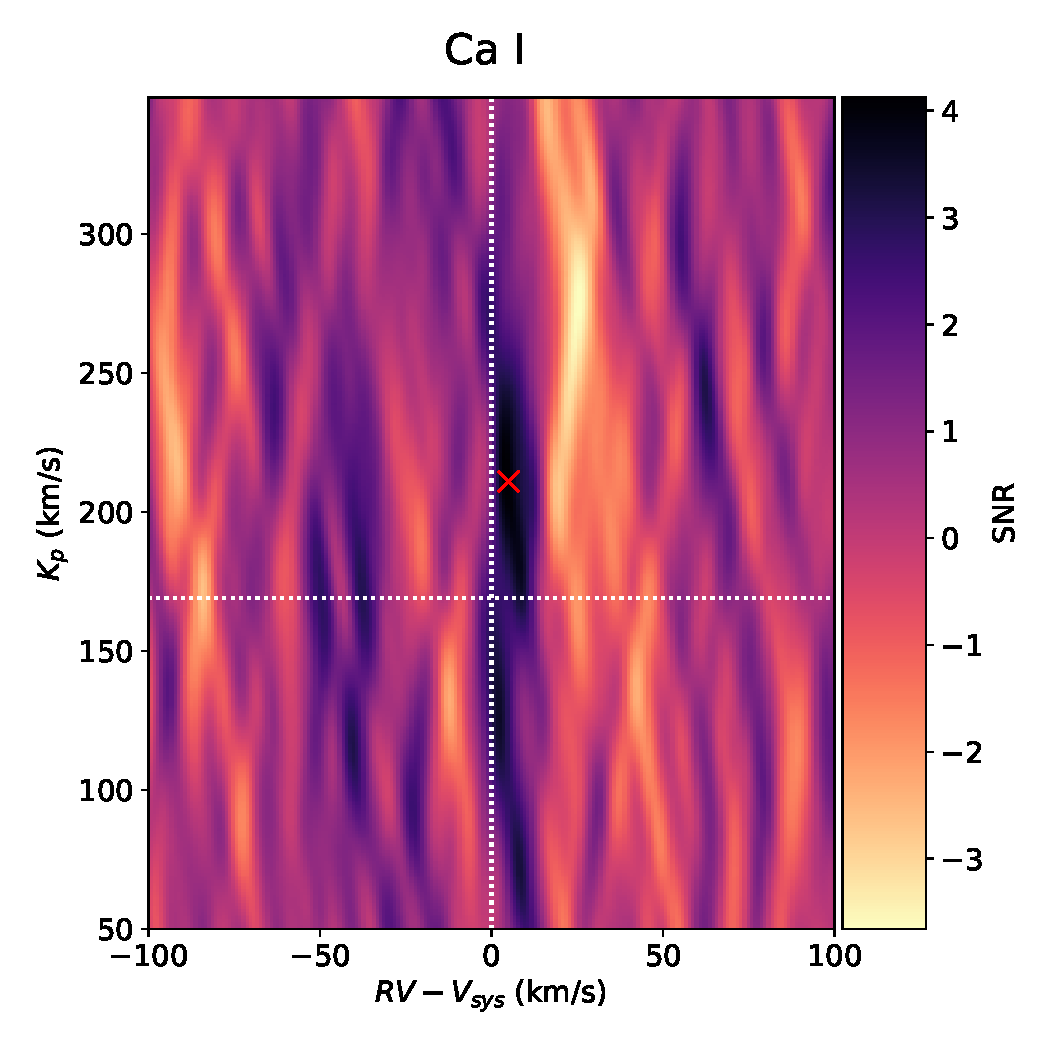
\includegraphics[width=\textwidth]{plots-updated/kp-vsys-map/blue/KELT-20b.20190504.blue.Ca.CCFs-shifted.pdf}
                
            \end{subfigure}
            \begin{subfigure}[b]{0.333\textwidth}\label{fig:1d-ccf-Ca-combined}
                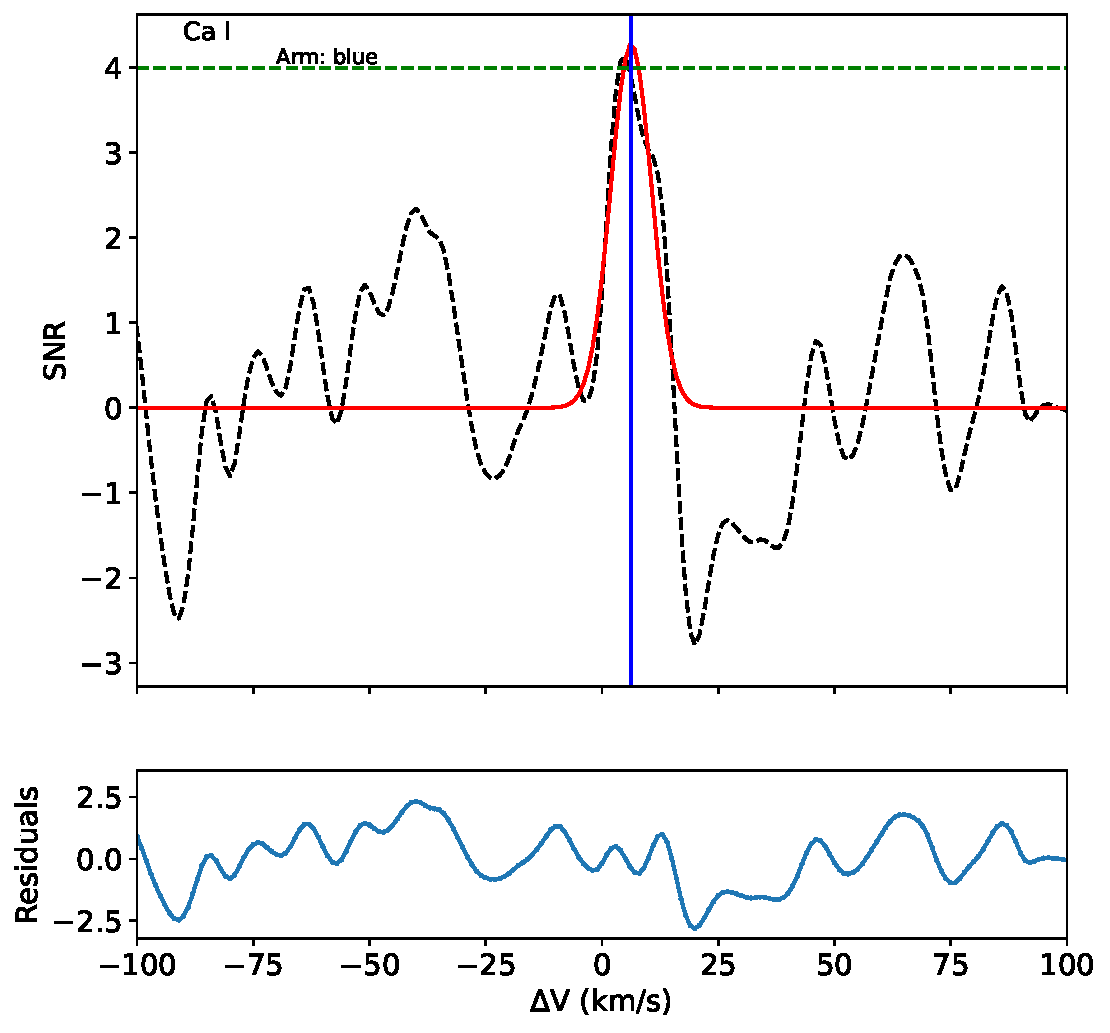
\includegraphics[width=\textwidth]{plots-updated/line-profile/blue/KELT-20b.20190504.blue.Ca.SNR-Gaussian.pdf}
                
            \end{subfigure}

            \begin{subfigure}[b]{0.333\textwidth}\label{fig:2d-ccf-Mn-combined}
                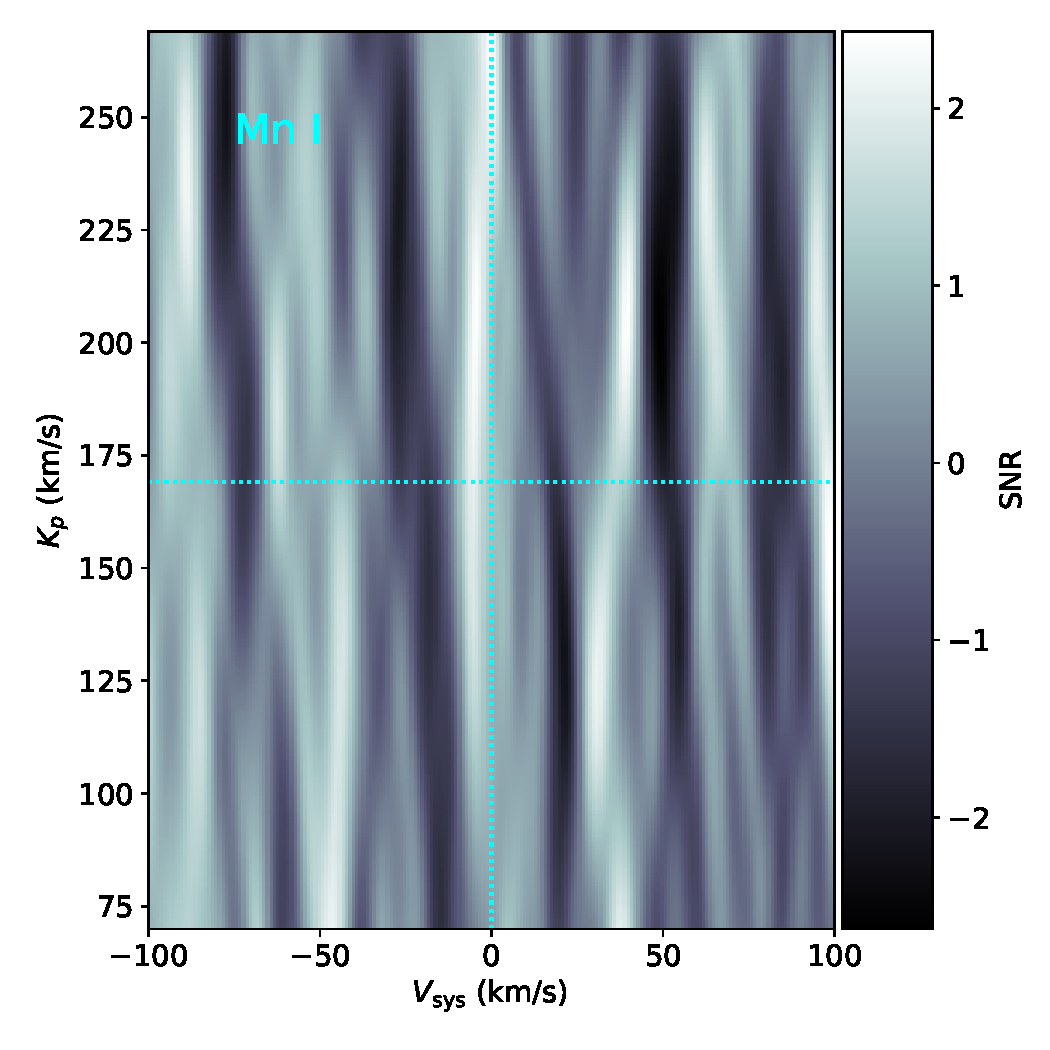
\includegraphics[width=\textwidth]{plots-updated/kp-vsys-map/blue/KELT-20b.20190504.blue.Mn.CCFs-shifted.pdf}
                
            \end{subfigure}
            \begin{subfigure}[b]{0.333\textwidth}\label{fig:1d-ccf-Mn-combined}
                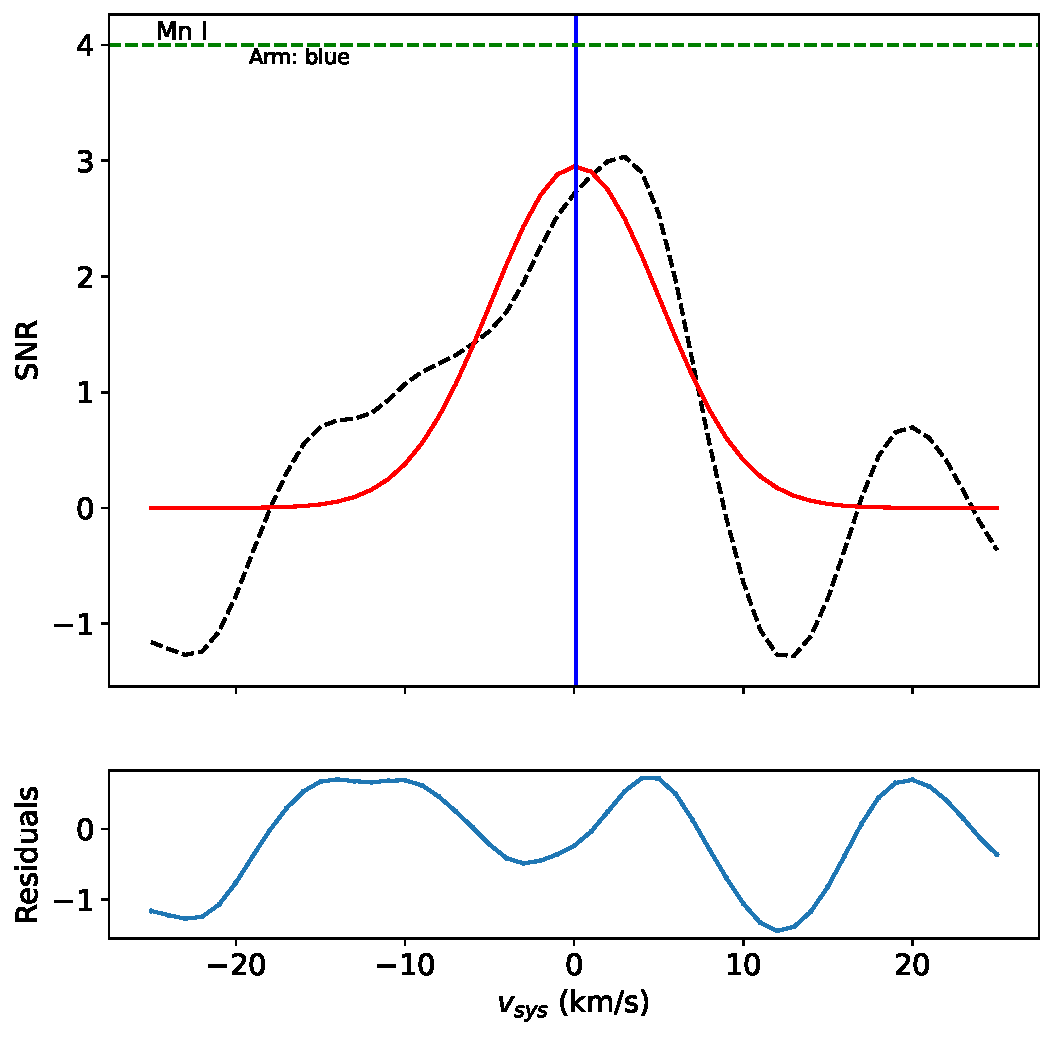
\includegraphics[width=\textwidth]{plots-updated/line-profile/blue/KELT-20b.20190504.blue.Mn.SNR-Gaussian.pdf}
                
            \end{subfigure}


        \caption{This figure shows the $K_p-v_{sys}$ maps, 1D CCFs, and line profiles for each species meeting the ${3\sigma}$ tentative detection threshold. The offset of the center of the 1D CCF Gaussian from the planetary rest frame, ${v_{sys}}=0$, denotes the line velocity. 
    }
        

        \end{figure*}



        % table showing summary of detections, tentative detections, and nondetections
            % detections are each species I find meeting detection threshold in red arm, blue arm, and combined arms
            % tentative detections are those meeting a 3- threshold in at least one arm of the PEPSI spectrograph AFTER ruling out spurious detections with both analysis of the RAW CCFs and running aliasing
        
            % table will include transmission VMR, recovered SNR, SNR found in other literaure and expected VMR, 
        \subsection{Detections and Nondetections}\label{subsec:Detections}
            We confirm previous detections of Fe I~\citep{Nugroho2020} and Fe II~\citep{CasasayasBarris2020, Nugroho2020, BelloArufe2022}. We tentatively confirm the previous detection of Na I~\citep{CasasayasBarris2020, Nugroho2020, Sicilia2022}. We present novel tentative detections of Co I, V I, and Ni I.

        
        \subsection{Atmospheric Dynamics}\label{subsec:Atmospheric Dynamics}
            % in desktop notes: reference the paper also finding offset of Fe I and II and its duscission of probing different pressures
            
            %Similar to the results in~\citep{Stangret2020}, we find a significant offset in $v_{sys}$ of Fe I and Fe II, suggesting we are probing different pressures in the atmosphere. Fe I's line velocity magnitude is greater than Fe II's across the entire transit, with a net blueshift with phase occurring in each species. As in~\citep{Stangret2020}, this result contradicts the discussion in~\citep{Gibson2020} and~\citep{Sing2019}.

            
        \begin{figure}[]\label{fig:FeI-II-Offset}
            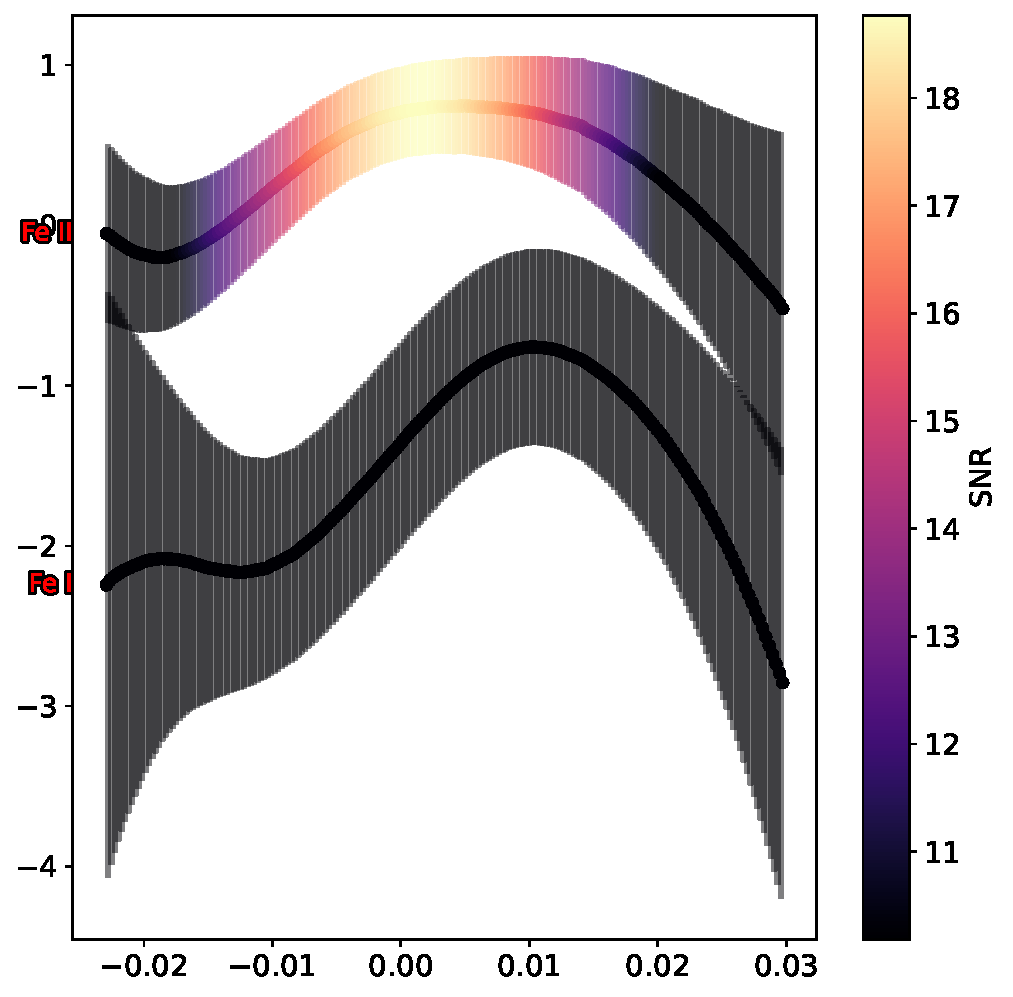
\includegraphics[width=0.45\textwidth]{plots/combined-phase-binned+RVs/KELT-20b.inverted-transmission-better.FeIFeII.CombinedWindCharacteristics_Combined.pdf}
            \caption{Phase-resolved Doppler shifts, or line profiles, of Fe I and Fe II during transit.}
            
        \end{figure}
        
        \begin{figure}[]\label{fig:VICaINaICoI-WindChars}
            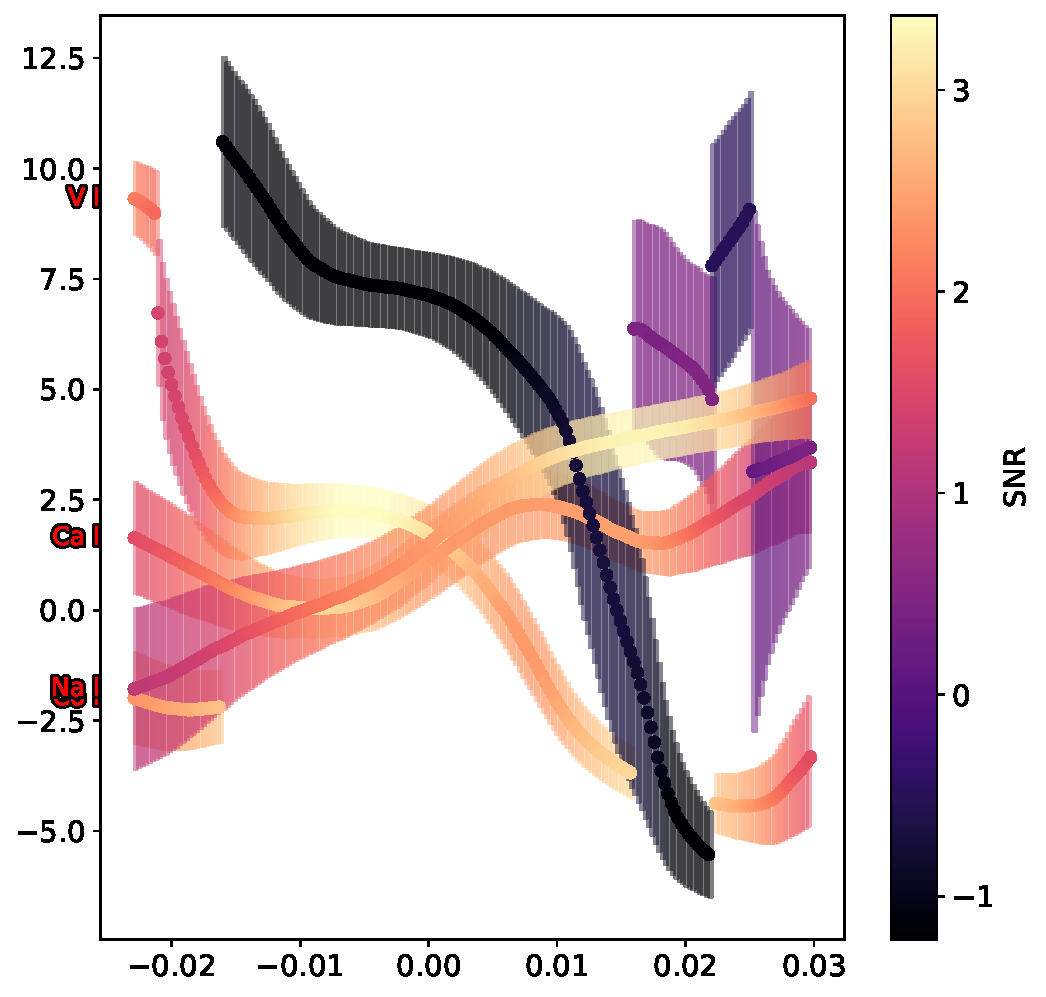
\includegraphics[width=0.45\textwidth]{plots/combined-phase-binned+RVs/KELT-20b.inverted-transmission-better.VICaINaICoI.CombinedWindCharacteristics_Combined.pdf}
            \caption{Phase-resolved Doppler shifts, or line profiles, of V I, Ca I, Na I, and Co I.}
            
        \end{figure}
        
        \begin{figure}[]\label{fig:combined-species-snr} 
            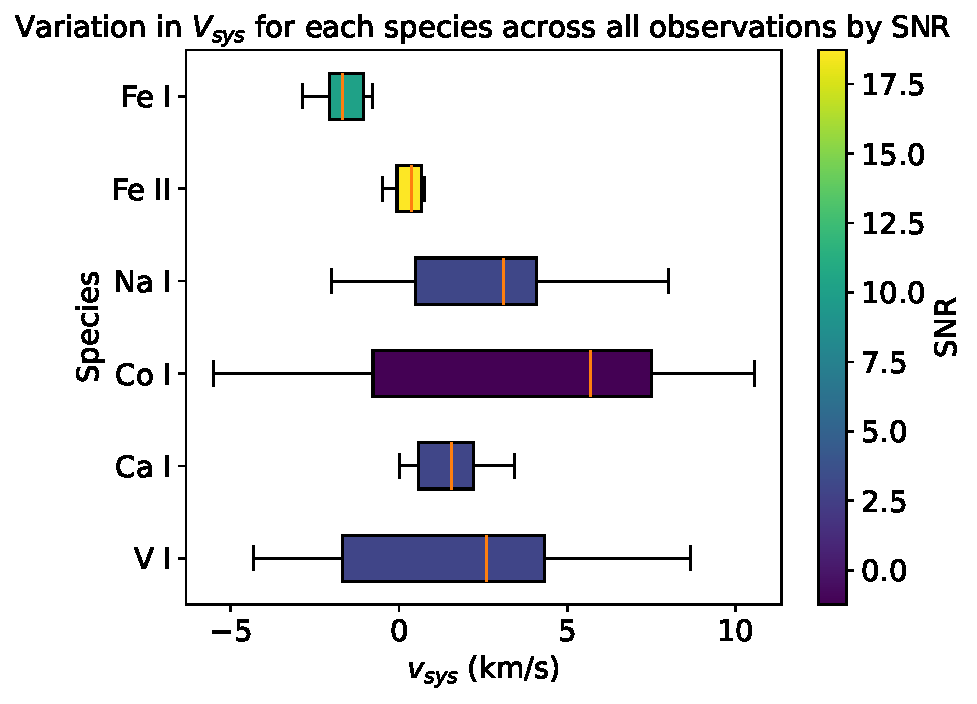
\includegraphics[width=0.45\textwidth]{plots/combined-species-snr/KELT-20b.inverted-transmission-better.CombinedSpeciesSNRs.pdf}
            \caption{The net Doppler shifts of each detected species, ordered and colored by their peak detection SNR.}
            
        \end{figure}

            The presence of neutral and singly-ionized iron in an UHJ atmosphere is expected, as the high temperature prevents its condensation.
        
        % in this section, I analyze the Vsys evolution of each species at least meeting the tentative detection threshold
            \subsubsection{Ingress/Egress Asymmetries}\label{subsubsec:Ingress/Egress Asymmetries}
                \begin{itemize}
                    \item 
                \end{itemize}
                
            \subsubsection{Line Profile Diagnostics}\label{subsubsec:Wind Profile Diagnostics}
                With the line behavior analyzed over the course of transit, we are left to attribute the observed asymmetries to several atmospheric equilibrium mechanisms. These include, but are not limited to, atmospheric escape, scale height differences, condensation, eccentricity, clouds, spatially varying winds, tidal deformation, and temperature-dependent opacity~\citep{Savel2023}. 

                When comparing our HRCCTS observations to models, our conclusions' validity are dependent on the accuracy of the atmospheric model. Given the impact that three-dimensional equilibrium processes, such as those mentioned above, have on $K_p-v_{sys}$ maps~\citep{Wardenier2021}, we wish to provide evidence for one or more of these proposed equilibrium mechanisms and constrain the three-dimensional behavior in the atmosphere for further study.

                % Similar discussion from paper on WASP-121b from V. Bourrier et al. (This paper is referenced in Savel et al. for the blueshifting CCF diagnostic, specifically atmospheric escape)
                    % DTN winds: The measured blueshift could trace fast winds going from the dayside to teh nightside along both terminators, as predicted for atmospheric ciruclation in the lower atmospheric layers of HJs. In this scenario the hotspot is expected to be located at the substellar point, as is indeed measured in the TESS phase curve of WASP-121b. -> Check from emission studies on KELT-20b the proposed location of the hotspot in relation to substellar point
                    % DTN Winds: It might be then expected that heat is efficiently redistibuted throug the fast DTN winds, whereas the phase curve indicates a strong temperature contrast -> Check the phase curve of KELT-20b and implications of temperature contrast across terminator
                    % DTN Winds: This might indicate that the iron signal arises form a different laer than those probed by the emission photometry. We may be probing layers at lower pressure than are probed by emission spectra, where the fast DTN winds homogenize temperature longitudinally. So the emission spectra are probing emission from high-altiude clods on the nightside, which would hide the emission from the deeper, hotter regions probed on the dayside.
                    % Clouds: It has been proposed that the nightsides of most UHJs are covered in clouds of similar composition, which would form at temperatures of arbout 1100K. With Tirr of 3310K, WASP-121b is in a regime where such clouds are not yet predicted to disperese (Keating et al. 2019) -> Check 
                    % Scale height differences: The measured bleushift could trace an anisoptropic expansion of the atmospheric layers, for exmaple, due to that asymmetrical irradiation of the dayside atmosphere or its compression by stellar wind and radiation.
                    % 3D simulations of the planetary atmosphere and more precise observatinos are required to explore the origin of the measured blueshift
                % Discussion from Kempton et al. 2012 (This paper is referenced in Savel et al. for blueshifting CCF diagnostic, specifically for scale height differences)
                    % We additionally explore the possibility of recovering the average terminator wind speed as a function of altitude by measuring Doppler shifts of individual spectral lines and spatially resolving wind speeds across the leading and trailing terminators during ingress and egress -> By comparing your CCFs between ingress and egress, you can potentially provide observational evidence alognside this modeled evidence
                    % The change of teh specific gas constant and its subsequent effect on the atmosphere's scale hei  ght likely significantly impacts the modeled transmission spectra of these GCMs. -> Examine the impact this has on your analysis given the scope, if any
                % Discussion from Wardenier et al. 2021 (This paper is referenced in Savel et al. for blueshifting CCF diagnostic, specifically for Weak Drag State)
                    % 
                % Discussion from Savel et al. 2022 (This paper is referenced in Savel et al. for blueshifting CCF diagnostic, specifically for Weak Drag State)

                % Discussion from Savel et al. 2022 (This paper is referenced in Savel et al. for blueshifting CCF diagnostic, specifically for cold interiors)
                
                % Discussion from Brogi et al. 2016 (This paper is referenced in Savel et al. for blueshifting CCF diagnostic, specifically for Superrotating jet)
                
                % Discussion from Ehrenreich et al. 2020 (This paper is referenced in Savel et al. for strongly blueshifting CCF diagnostic, specifically for Condensation)

                % Discussion from Kempten and Rauscher 2012 (This paper is referenced in Savel et al. 2023 for varying Doppler shift over phase diagnostic and comparison of ingress/egress Doppler shifts and comparison of Doppler shifts of different-strength lines, specifically for spatially varying winds)
                    % 
                % Discussion from Wardenier et al. 2021 (This paper is referenced in Savel et al. 2023 for blueshifting CCF over phase, specifically for T-dependent opacity)
                    
        % in this section I will attempt to connect the observed asymmetrical behavior of each species 1d CCF profile to proposed limb asymmetry mechanisms using Savel et al 2023
        \subsection{Nondetections}\label{subsec:Nondetections}

    \section{Conclusions}\label{sec:Conclusions}


    \vspace{5mm}
    \facilities{LBT}

    \software{astropy \citep{2013A&A...558A..33A,2018AJ....156..123A}, 
            Jupyter \citep{jupyter},
            matplotlib \citep{Matplotlib},
            molecfit \citep{Kausch2015, Smette2015},
            numpy \citep{NumPy},
            petitRADTRANS \citep{petitRADTRANS},
            PyFastChem \citep{PyFastChem},
            uncertainties~\citet{uncertainties}
            }

    %% Appendix material should be preceded with a single \appendix command.
    %% There should be a \section command for each appendix. Mark appendix
    %% subsections with the same markup you use in the main body of the paper.

    %% Each Appendix (indicated with \section) will be lettered A, B, C, etc.
    %% The equation counter will reset when it encounters the \appendix
    %% command and will number appendix equations (A1), (A2), etc. The
    %% Figure and Table counter will not reset.
    \clearpage
    \bibliography{bibliography}{}
    \bibliographystyle{aasjournal}

    \appendix  
        \section{Model transmission spectra}
            \begin{figure*}[ht!]
                \centering
                \begin{subfigure}[b]{0.3\textwidth}\label{fig:Fe-spectrum}
                    \centering
                    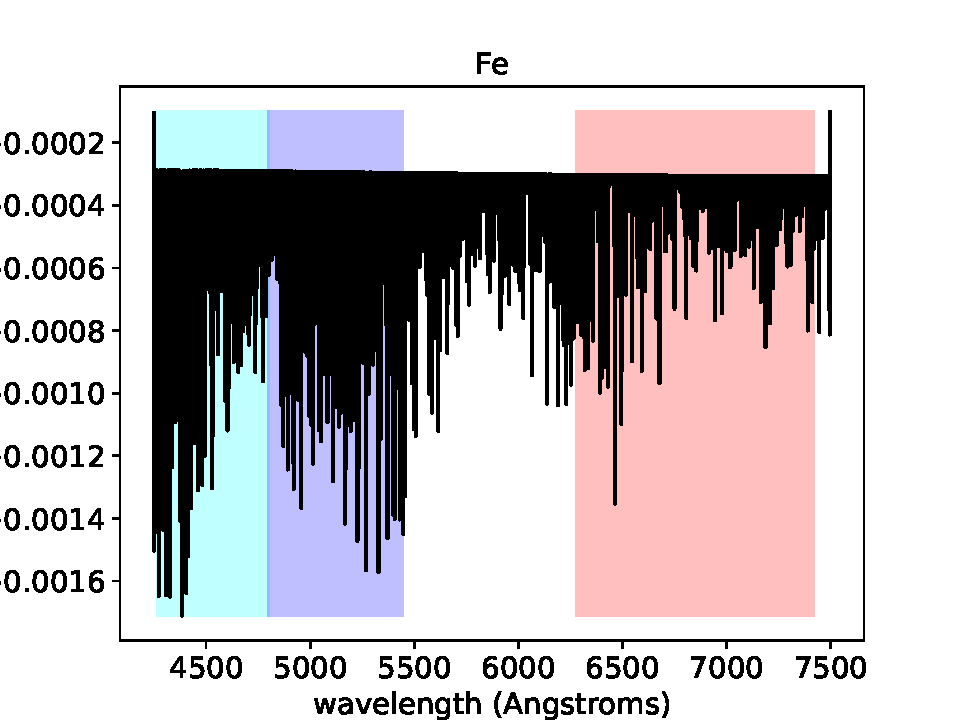
\includegraphics[width=\textwidth]{plots/spectra/spectrum.KELT-20b.Fe.5.39e-05.inverted-transmission-better}
                    
                \end{subfigure}
                \begin{subfigure}[b]{0.3\textwidth}\label{fig:Fe+-spectrum
                    \centering
                    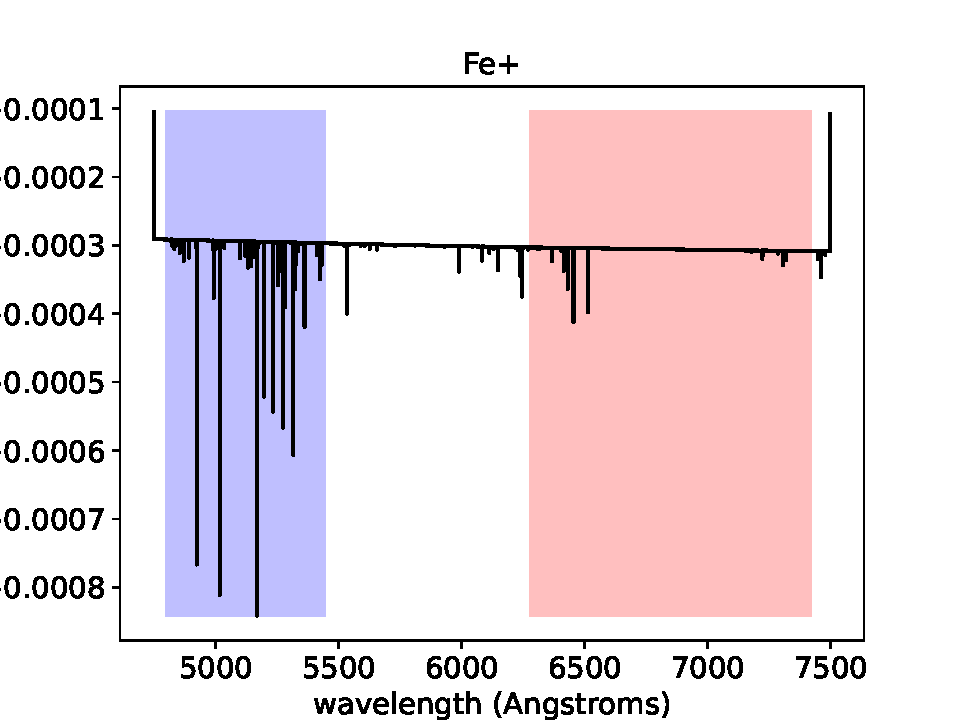
\includegraphics[width=\textwidth]{plots/spectra/spectrum.KELT-20b.Fe+.5.39e-05.inverted-transmission-better.pdf}
                    }
                \end{subfigure}
                \begin{subfigure}[b]{0.3\textwidth}\label{fig:Na-spectrum}
                    \centering
                    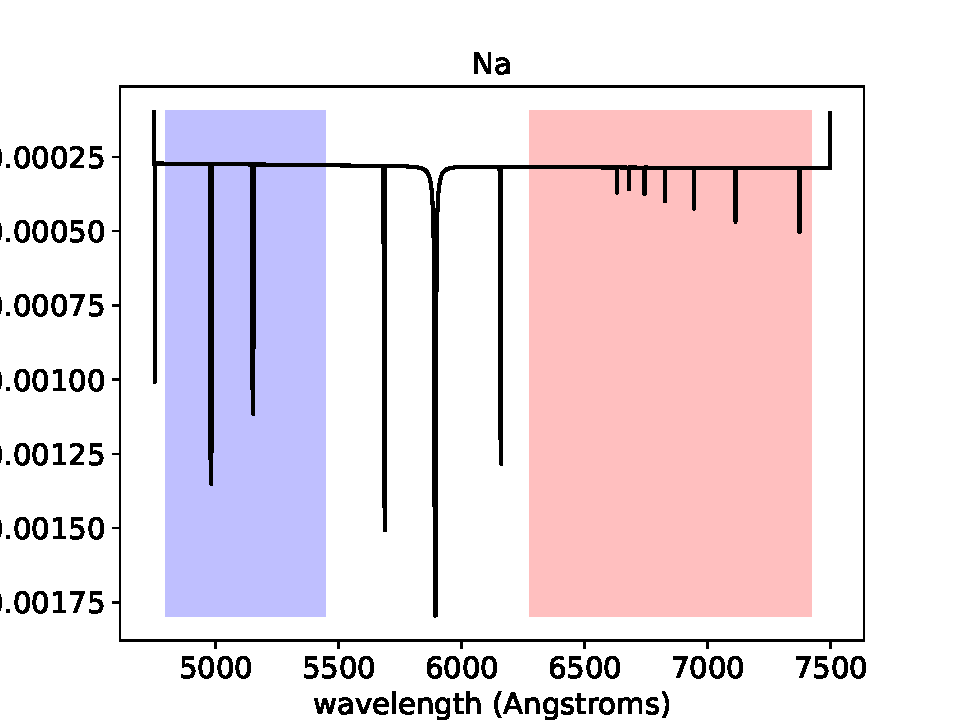
\includegraphics[width=\textwidth]{plots/spectra/spectrum.KELT-20b.Na.2.94e-06.inverted-transmission-better.pdf}
                    
                \end{subfigure}
                \begin{subfigure}[b]{0.3\textwidth}\label{fig:Co-spectrum}
                    \centering
                    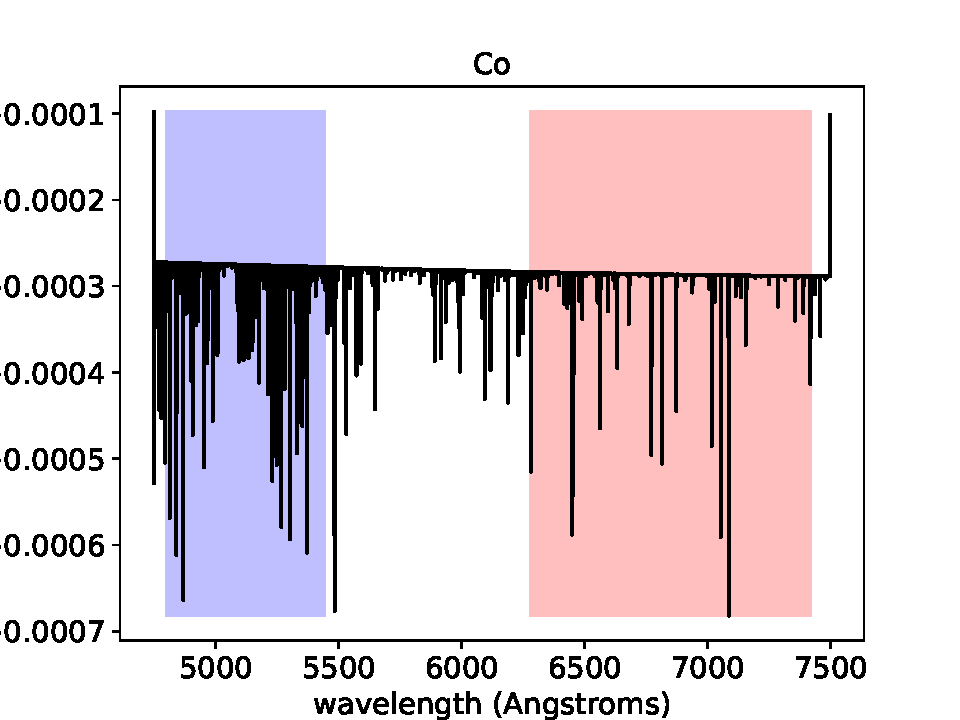
\includegraphics[width=\textwidth]{plots/spectra/spectrum.KELT-20b.Co.1.67e-07.inverted-transmission-better.pdf}
                    
                \end{subfigure}
                \begin{subfigure}[b]{0.3\textwidth}\label{fig:V-spectrum}
                    \centering
                    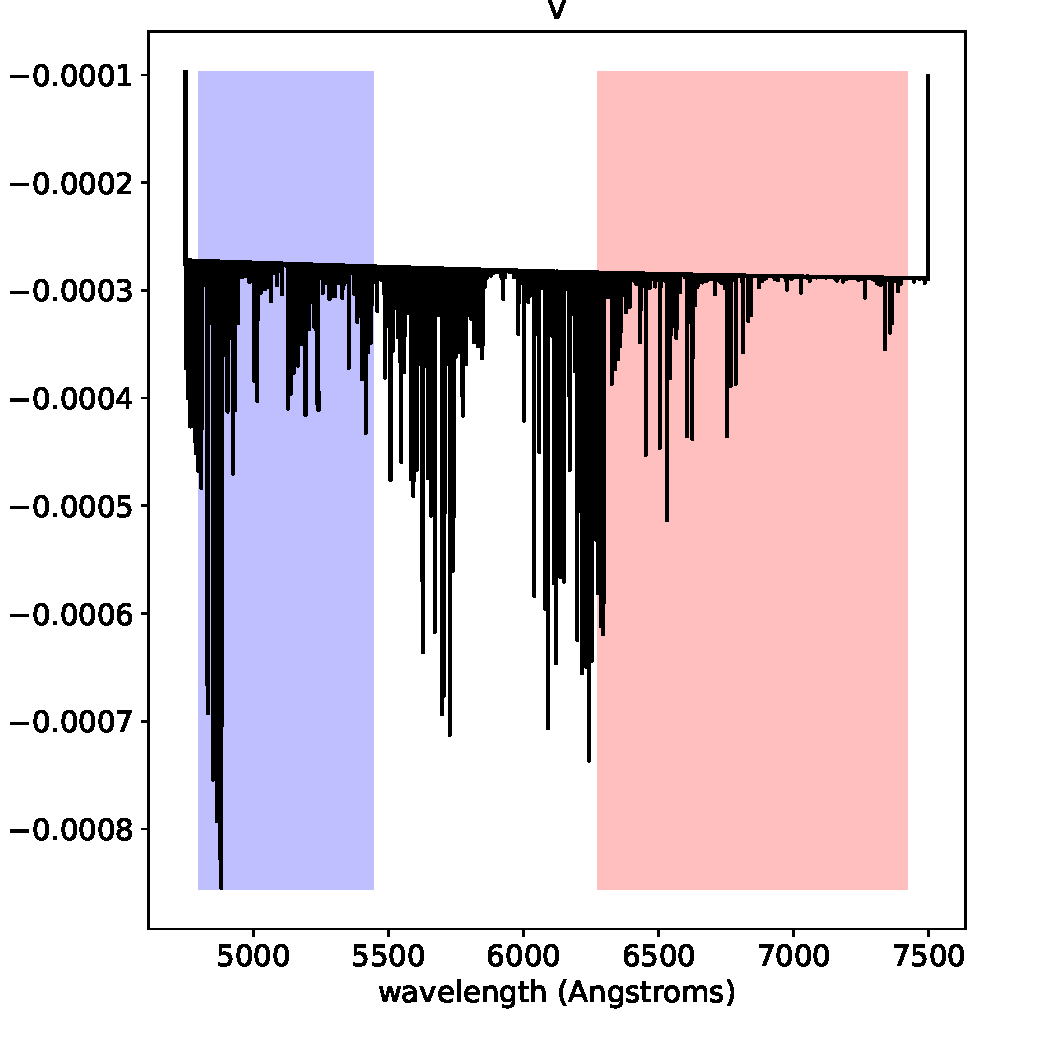
\includegraphics[width=\textwidth]{plots/spectra/spectrum.KELT-20b.V.5.623e-09.inverted-transmission-better.pdf}
                    
                \end{subfigure}
                \begin{subfigure}[b]{0.3\textwidth}\label{fig:Ca-spectrum}
                    \centering
                    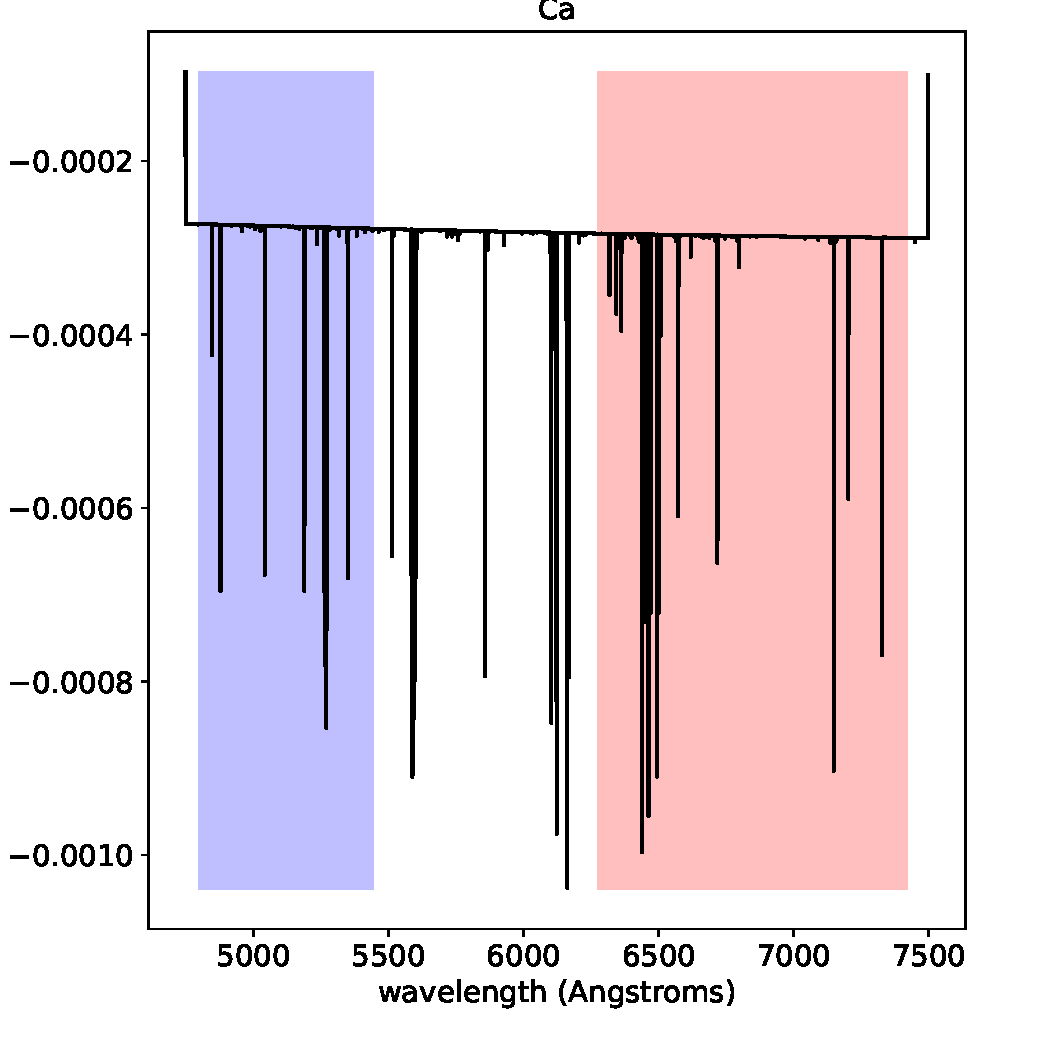
\includegraphics[width=\textwidth]{plots/spectra/spectrum.KELT-20b.Ca.2.101e-08.inverted-transmission-better.pdf}
                    
                \end{subfigure}\label{fig:main-spectra}
                % Add additional subfigures as needed
                \caption{Model transmission spectra generated by \code{petitRADTRANS}, with the wavelengths covered by PEPSI's arms shown in blue and red, respectively.}
                
            \end{figure*}
        
        \section{Line Profiles}
            \begin{figure*}[ht!]\label{fig:line-profle-overlaid-arms}
                \begin{subfigure}[b]{0.3\textwidth}
                    \centering
                    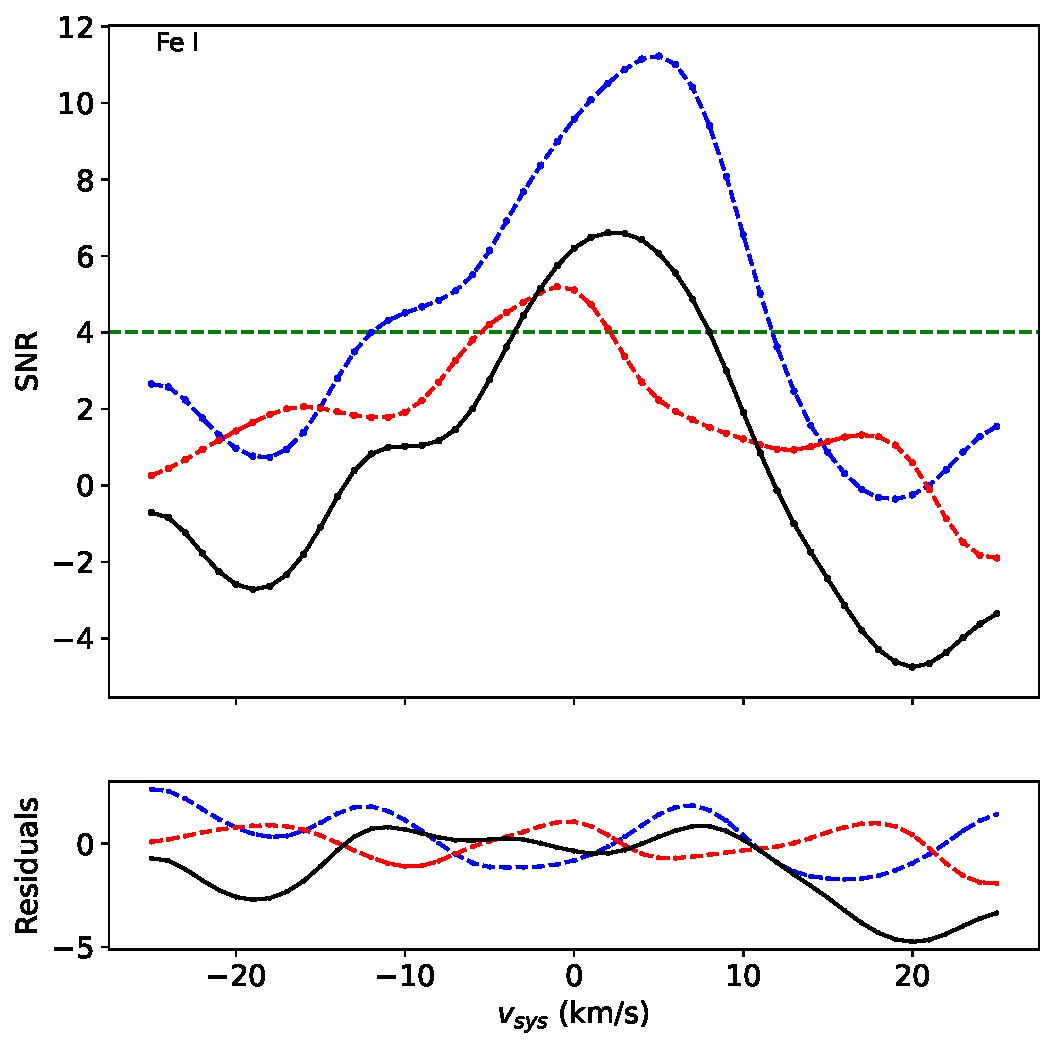
\includegraphics[width=\textwidth]{plots-updated/line-profile-overlaidarms/KELT-20b.20190504.combined.Fe I.line-profiles-overlaidarms.pdf}
                \end{subfigure}
                \begin{subfigure}[b]{0.3\textwidth}
                    \centering
                    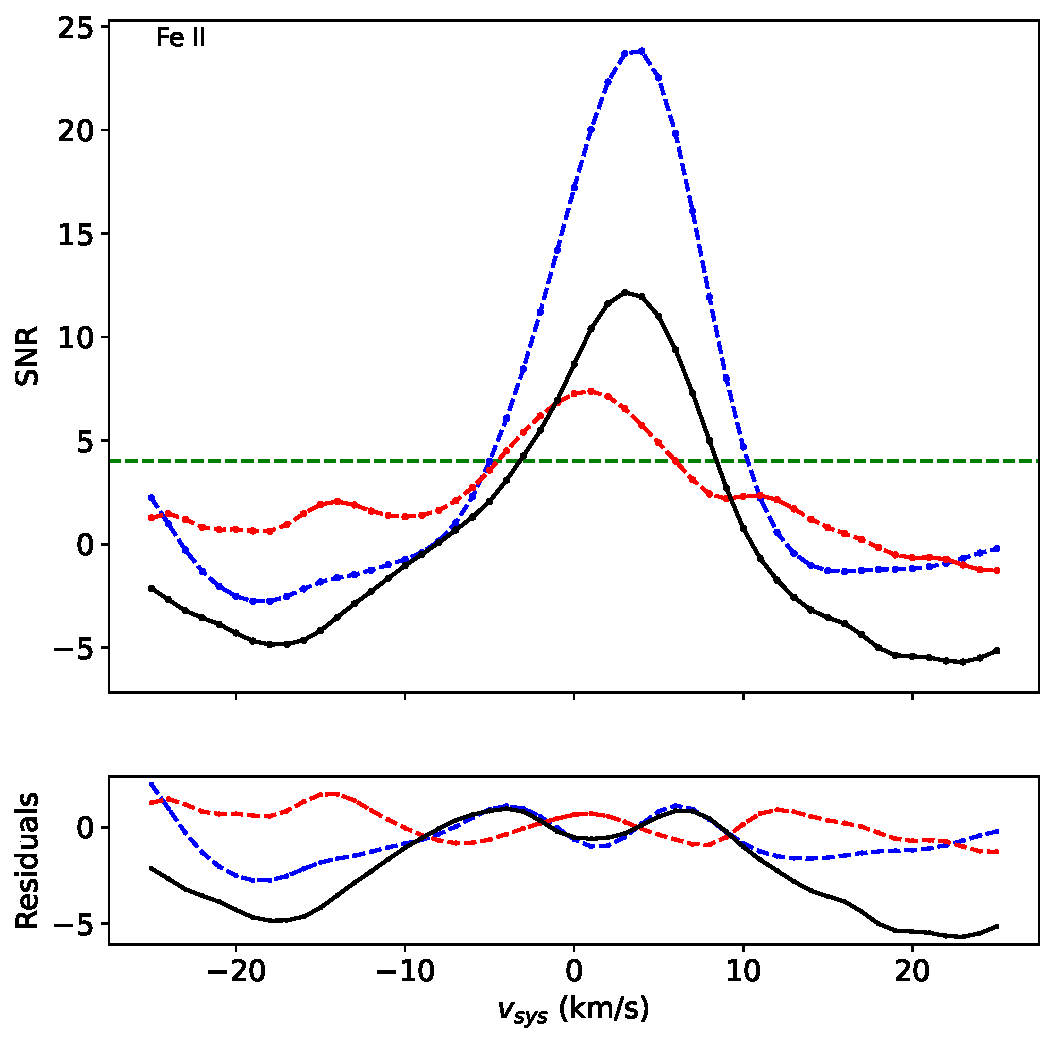
\includegraphics[width=\textwidth]{plots-updated/line-profile-overlaidarms/KELT-20b.20190504.combined.Fe II.line-profiles-overlaidarms.pdf}
                \end{subfigure}
                \begin{subfigure}[b]{0.3\textwidth}
                    \centering
                    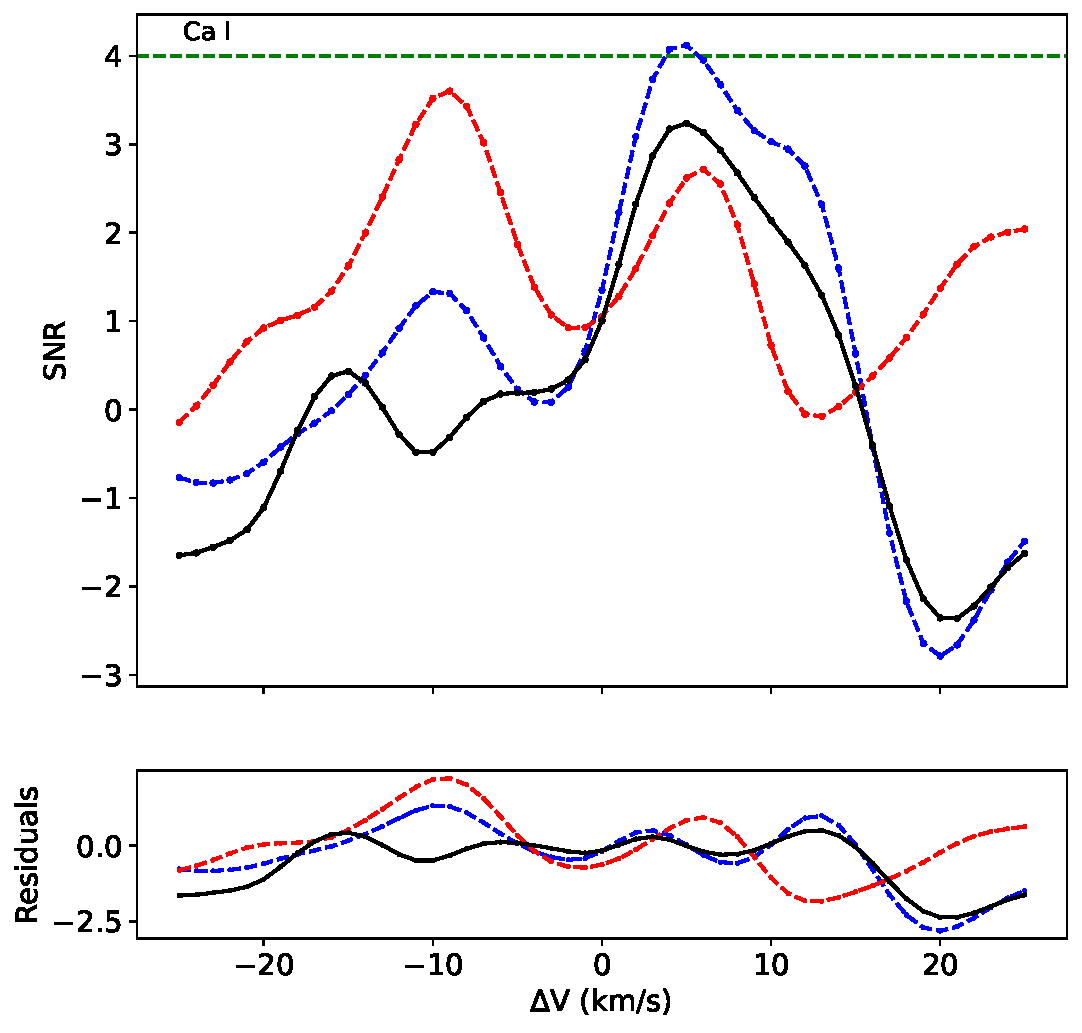
\includegraphics[width=\textwidth]{plots-updated/line-profile-overlaidarms/KELT-20b.20190504.combined.Ca I.line-profiles-overlaidarms.pdf}
                \end{subfigure}
                \begin{subfigure}[b]{0.3\textwidth}
                    \centering
                    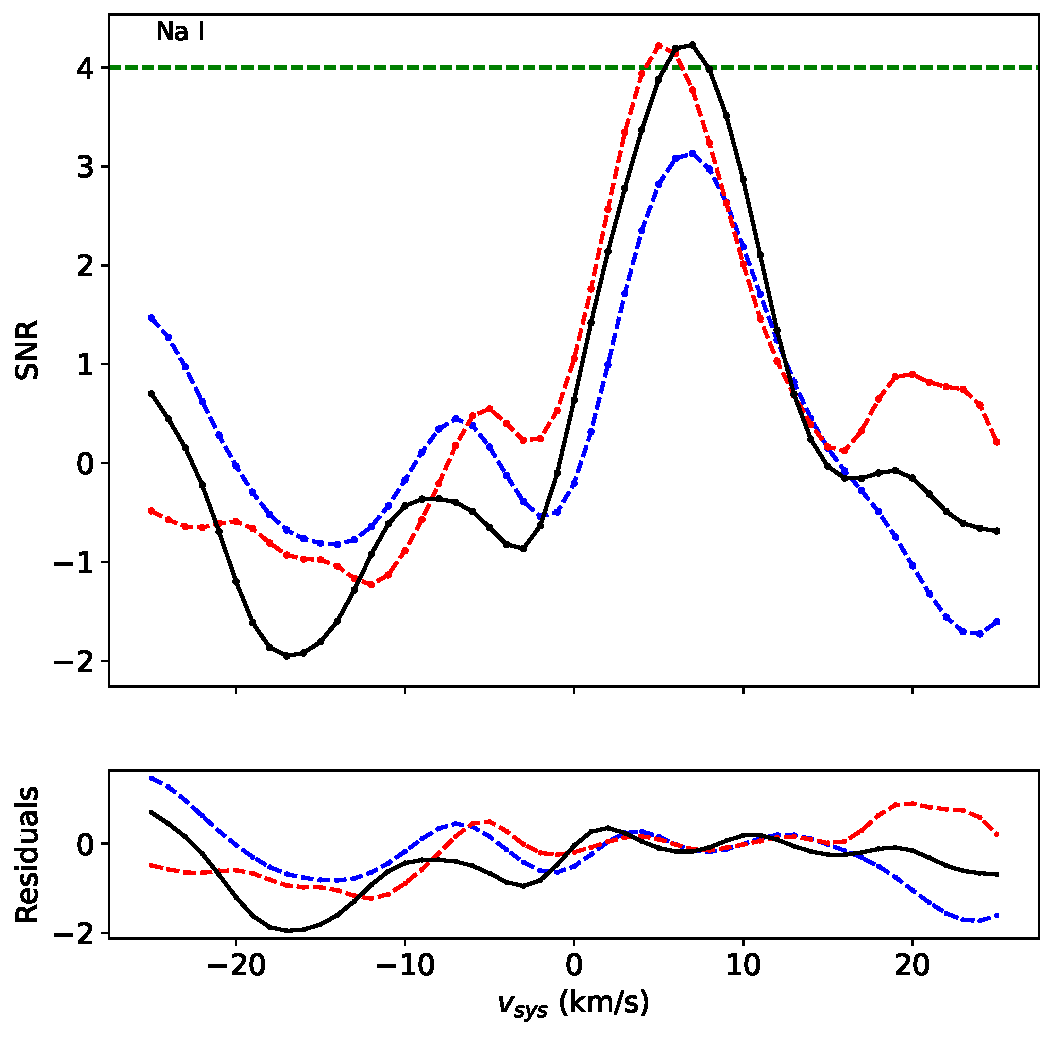
\includegraphics[width=\textwidth]{plots-updated/line-profile-overlaidarms/KELT-20b.20190504.combined.Na I.line-profiles-overlaidarms.pdf}
                \end{subfigure}
                \begin{subfigure}[b]{0.3\textwidth}
                    \centering
                    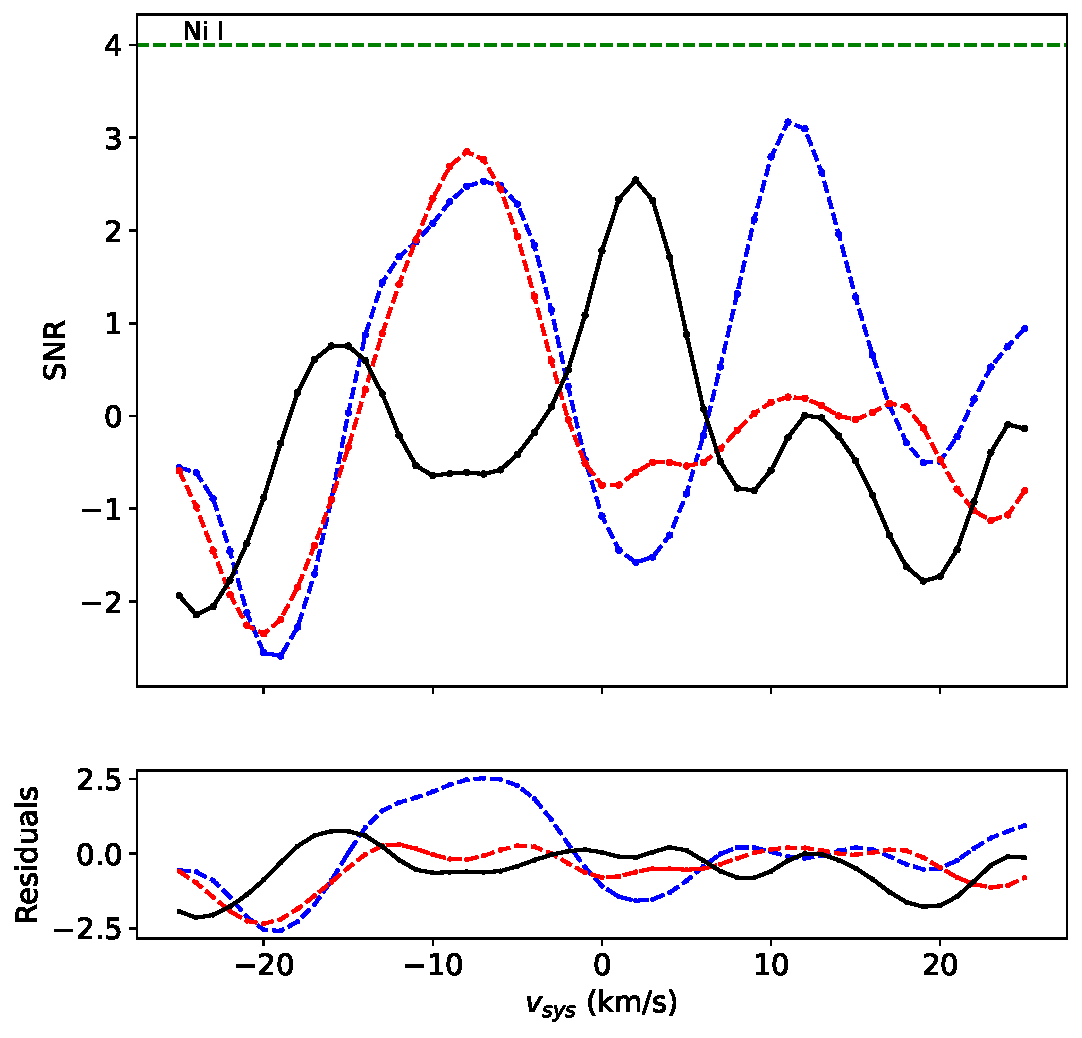
\includegraphics[width=\textwidth]{plots-updated/line-profile-overlaidarms/KELT-20b.20190504.combined.Ni I.line-profiles-overlaidarms.pdf}
                \end{subfigure}
                \caption{}
                
            \end{figure*}

        \section{$K_p$-$v_{sys}$ Maps}
            \begin{figure*}[ht!]\label{fig:kp-vsys-maps}
                \begin{subfigure}[b]{0.3\textwidth}
                    \centering
                    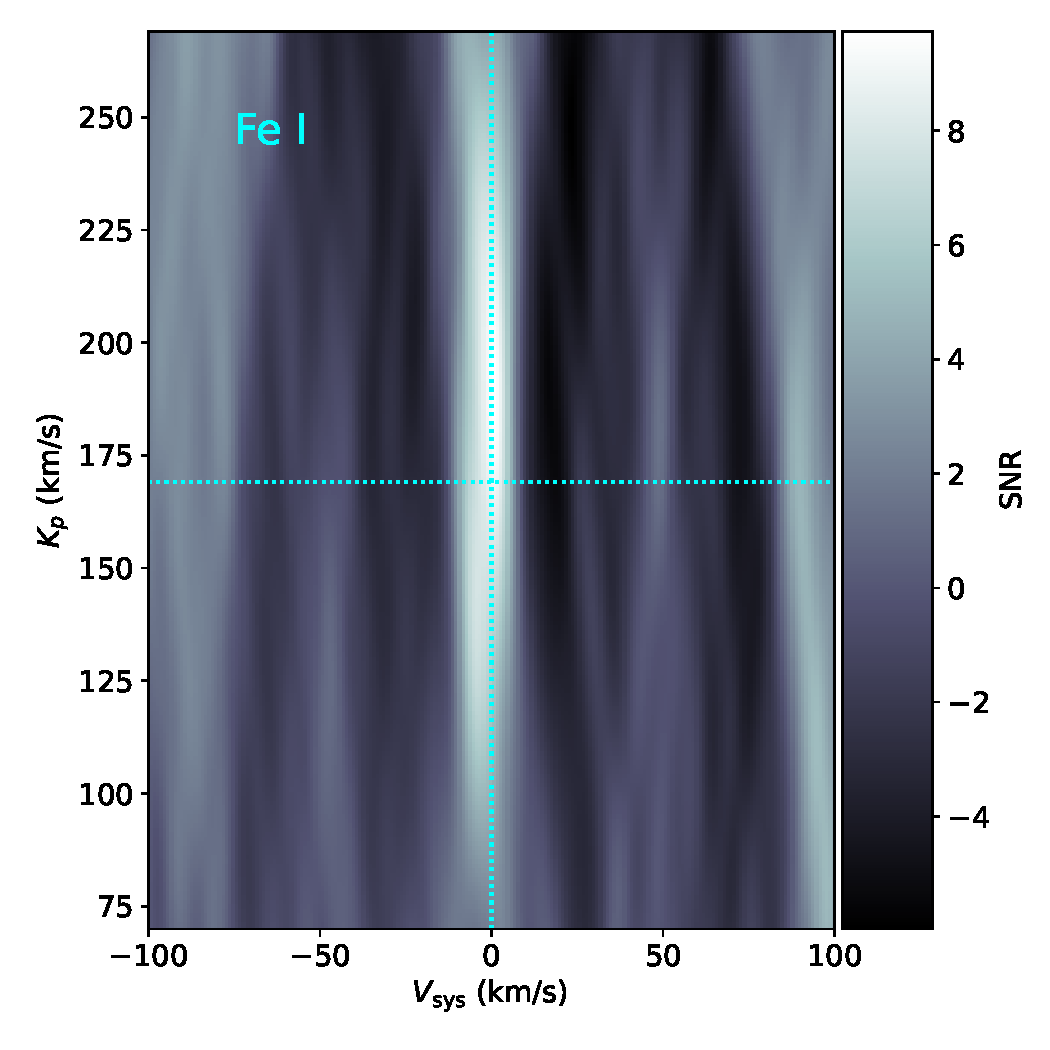
\includegraphics[width=\textwidth]{plots-updated/kp-vsys-map/combined/KELT-20b.20190504.combined.Fe.CCFs-shifted.pdf}
                \end{subfigure}
                \begin{subfigure}[b]{0.3\textwidth}
                    \centering
                    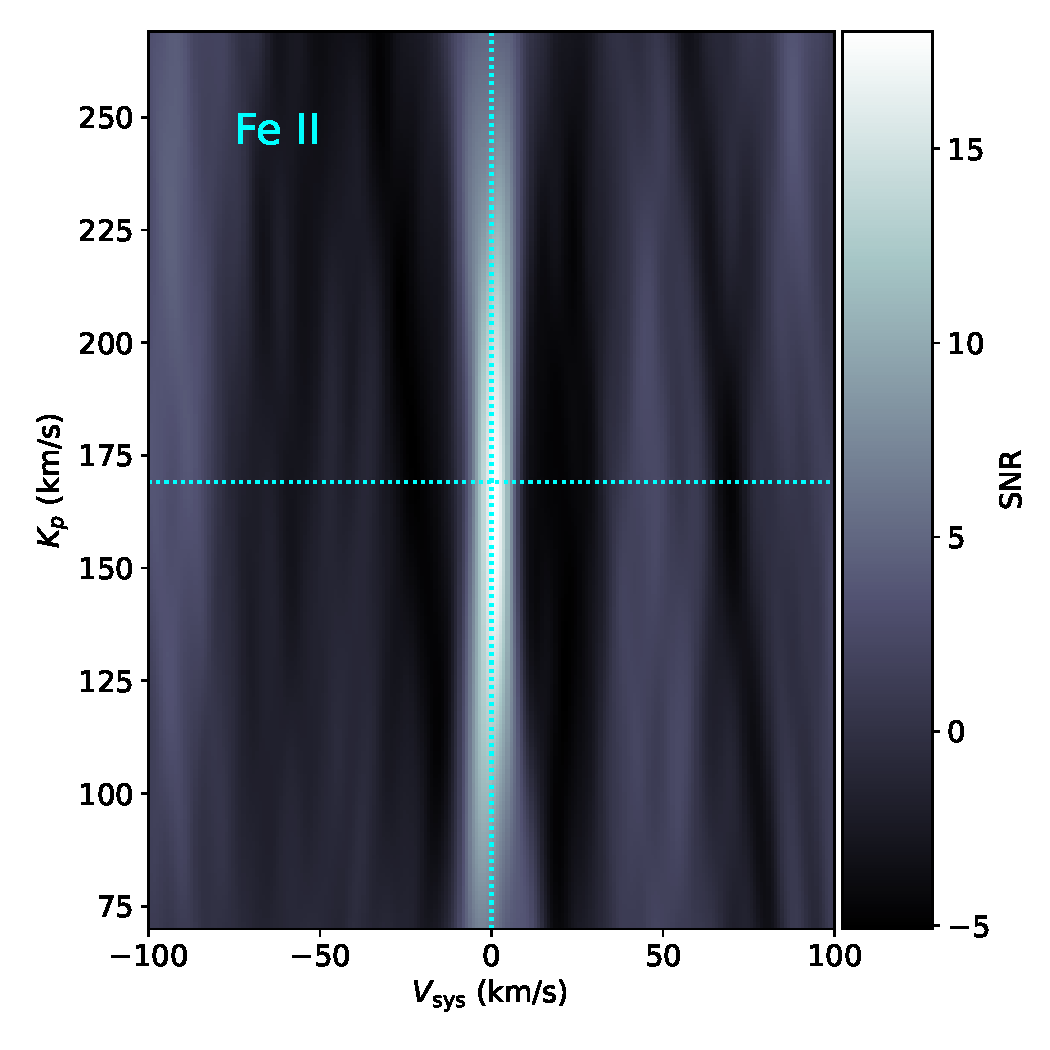
\includegraphics[width=\textwidth]{plots-updated/kp-vsys-map/combined/KELT-20b.20190504.combined.Fe+.CCFs-shifted.pdf}
                \end{subfigure}
                \begin{subfigure}[b]{0.3\textwidth}
                    \centering
                    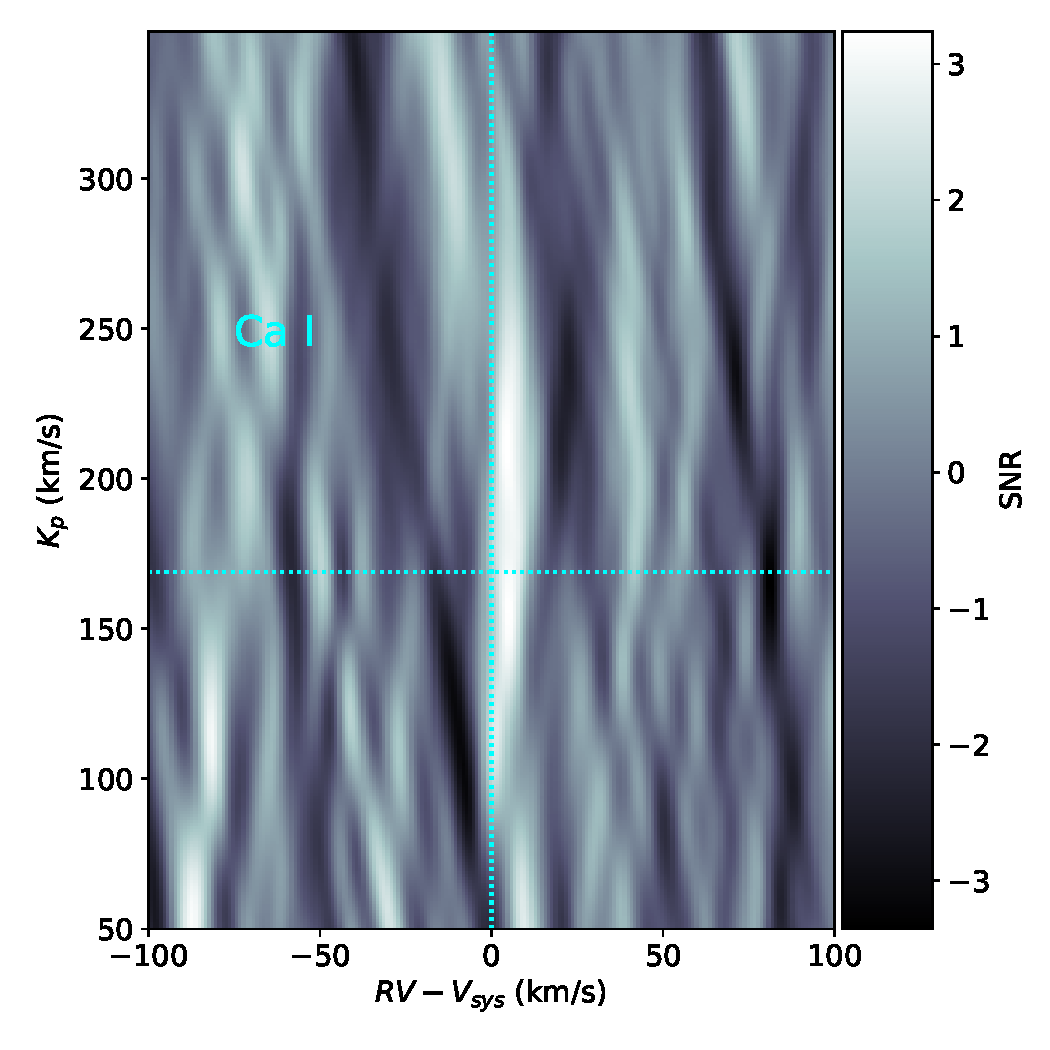
\includegraphics[width=\textwidth]{plots-updated/kp-vsys-map/combined/KELT-20b.20190504.combined.Ca.CCFs-shifted.pdf}
                \end{subfigure}
                \begin{subfigure}[b]{0.3\textwidth}
                    \centering
                    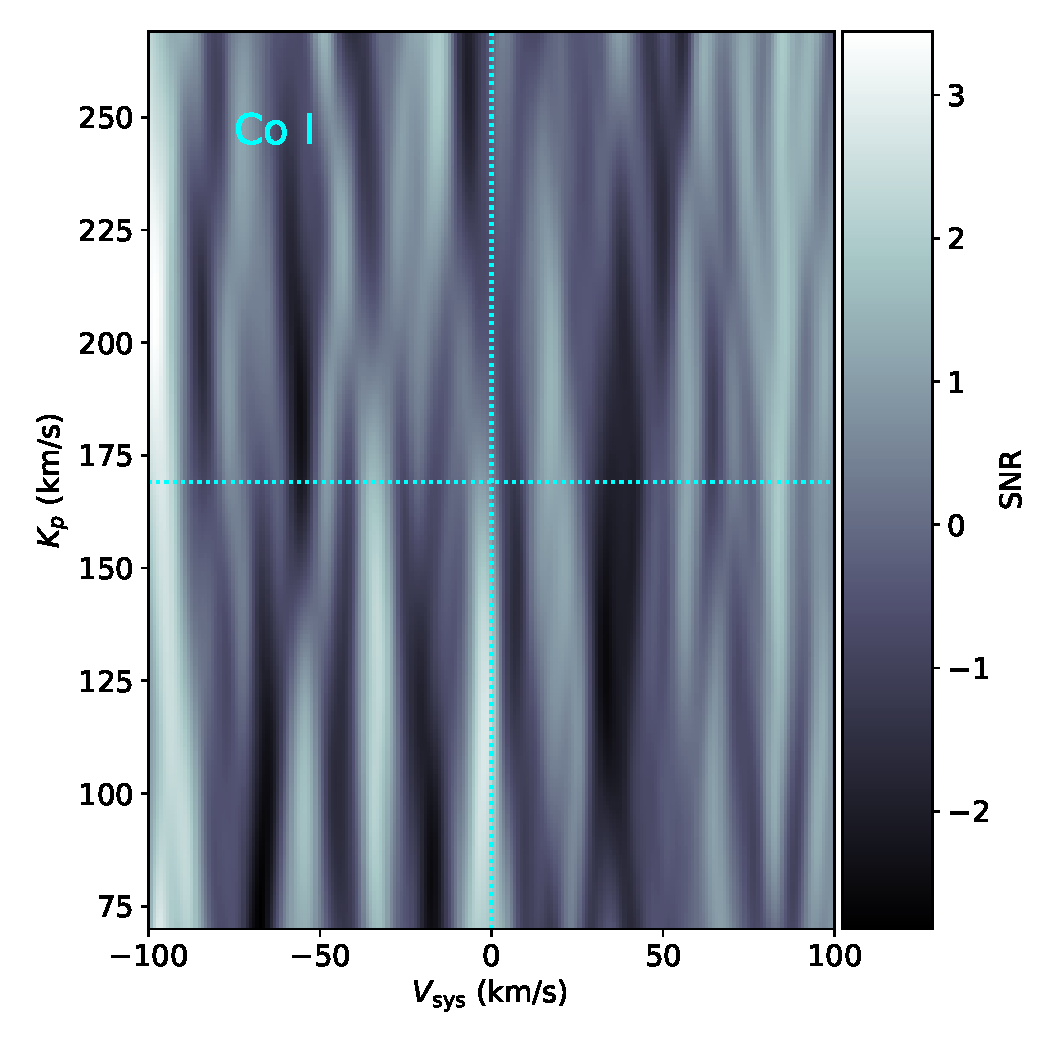
\includegraphics[width=\textwidth]{plots-updated/kp-vsys-map/combined/KELT-20b.20190504.combined.Co.CCFs-shifted.pdf}
                \end{subfigure}
                \begin{subfigure}[b]{0.3\textwidth}
                    \centering
                    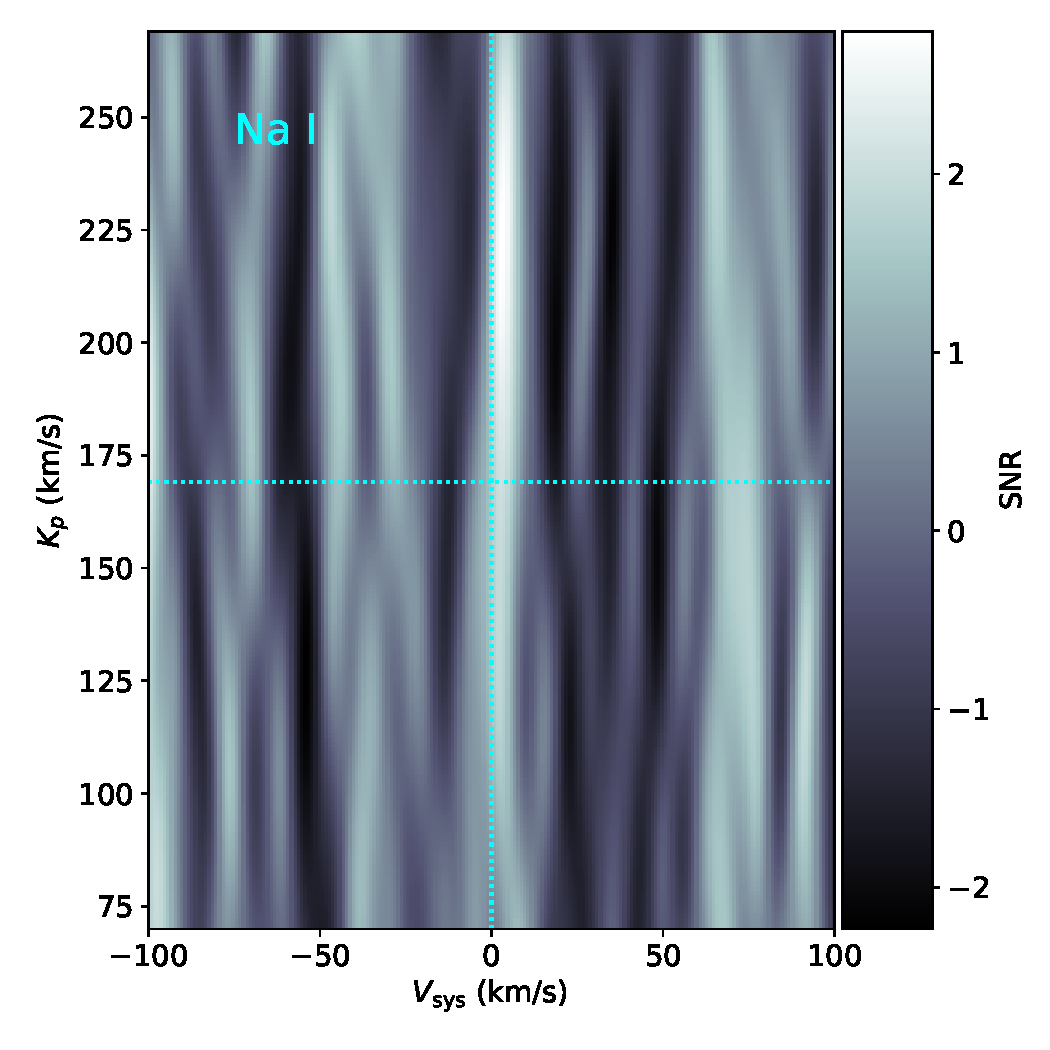
\includegraphics[width=\textwidth]{plots-updated/kp-vsys-map/combined/KELT-20b.20190504.combined.Na.CCFs-shifted.pdf}
                \end{subfigure}
                \caption{}
            \end{figure*}

        \section{Phase Resolved Line Profiles}
        
        
\end{document}